\documentclass[10pt,journal,compsoc]{IEEEtran}
\usepackage{wrapfig}
 \usepackage{amsmath}
 \usepackage{url}
 \usepackage{pifont}
\usepackage{rotating}
%\usepackage{balance} 
\usepackage{color, colortbl}
\usepackage{graphicx}
\usepackage{algorithmicx}
\usepackage{program}
\usepackage{cite}
\usepackage{alltt}
\newcommand{\eq}[1]{Equation~\ref{eq:#1}}
\newcommand{\bi}{\begin{itemize}}
\newcommand{\ei}{\end{itemize}}
\newcommand{\be}{\begin{enumerate}}
\newcommand{\ee}{\end{enumerate}}
\newcommand{\tion}[1]{\textsection\ref{sec:#1}}
\newcommand{\fig}[1]{Figure~\ref{fig:#1}}
\definecolor{lightgray}{gray}{0.975}
\usepackage{fancyvrb}
\usepackage{stfloats}
\usepackage{multirow}
\usepackage{listings}
\usepackage{amsmath} 
\DeclareMathOperator*{\argmin}{arg\,min} 
\DeclareMathOperator*{\argmax}{arg\,max} 


\definecolor{darkgreen}{rgb}{0,0.3,0}

\usepackage[table]{xcolor}
\definecolor{Gray}{rgb}{0.88,1,1}
\definecolor{Gray}{gray}{0.85}
\definecolor{Blue}{RGB}{0,29,193}
\newcommand{\G}{\cellcolor{green}}
\newcommand{\Y}{\cellcolor{yellow}}


\definecolor{MyDarkBlue}{rgb}{0,0.08,0.45} 
\newenvironment{changed}{\par\color{MyDarkBlue}}{\par}

\newcommand{\ADD}[1]{\textcolor{MyDarkBlue}{{\bf #1}}}
\newcommand{\addit}[1]{\begin{changed}\input{#1}\end{changed}}

\begin{document}

\title{GALE: Geometric Active Learning \\ for Search-Based Software Engineering}

\author{
Joseph~Krall\thanks{Joseph Krall is a postdoc at LoadIQ, Nevada, USA; email:  kralljoe@gmail.com.},
Tim~Menzies,~\IEEEmembership{Member,~IEEE},\thanks{
Tim Menzies
is with Computer Science, North Carolina State University, USA; e-mail: tim.menzies@gmail.com.}
Misty Davies~\IEEEmembership{Member,~IEEE}
\thanks{
Misty Davies is with the Intelligent Systems Division,
NASA Ames Research Center, CA, USA;
e-mail:
misty.d.davies@nasa.gov.}
}

\IEEEcompsoctitleabstractindextext{%
\begin{abstract}
Multi-objective evolutionary algorithms (MOEAs)
help software engineers
find novel solutions to complex problems. When
\ADD{automatic tools} explore too many options, they are 
slow to use and  hard to comprehend.
GALE is a  near-linear time MOEA that builds
a piecewise approximation 
to the surface of best solutions along the Pareto frontier.
For each piece,
GALE mutates solutions towards the better end.
In numerous case studies, 
GALE finds comparable solutions to standard methods
(NSGA-II, SPEA2) using far fewer evaluations (e.g.
20 evaluations, not 1000).
GALE is recommended when a
 model is expensive to evaluate, or when
some audience needs to browse and understand
how an MOEA has made its conclusions.

\end{abstract}

\begin{keywords}
Multi-objective optimization, Search based software engineering, Active Learning
\end{keywords}}

\maketitle

\markboth{Name of Journal here,~Vol.~X, No.~Y, January~2014}%
{Shell \MakeLowercase{\textit{et al.}}: Accelerated Active Learning for Search Based Software Engineering}


\IEEEdisplaynotcompsoctitleabstractindextext
\IEEEpeerreviewmaketitle



\section{Introduction}
\ADD{Given recent advances in computing hardware},  
software analysts can use automatic tools to
explore thousands to millions
of options of their systems. 
Such tools work at different speeds than humans.  Valerdi notes that it can take days for
human experts to review just a few dozen
examples~\cite{valerdi11}.  In that same time, an
automatic tool can explore thousands to millions to
billions more solutions.  
It is an overwhelming task for humans to
certify the correctness of conclusions generated
from so many results. Verrappa and Letier warn that
\begin{quote}
``..for industrial problems, these algorithms generate
(many) solutions, which makes the tasks of
understanding them and selecting one among them
difficult and time consuming''~\cite{veer11}.
\end{quote}
%% This is a problem since for many human-in-the-loop situations,
%% tools must be designed such that managers can debate their results
%% (e.g. to decide if it is wise
%% to deploy the results as a change to their
%% processes). 
%% \ADD{In our experience, 
%% to better support debates during decision making,
%% it is wise to
%% reducing the number of options business users
%% have to consider.}

%% \begin{figure}[!b]
%% 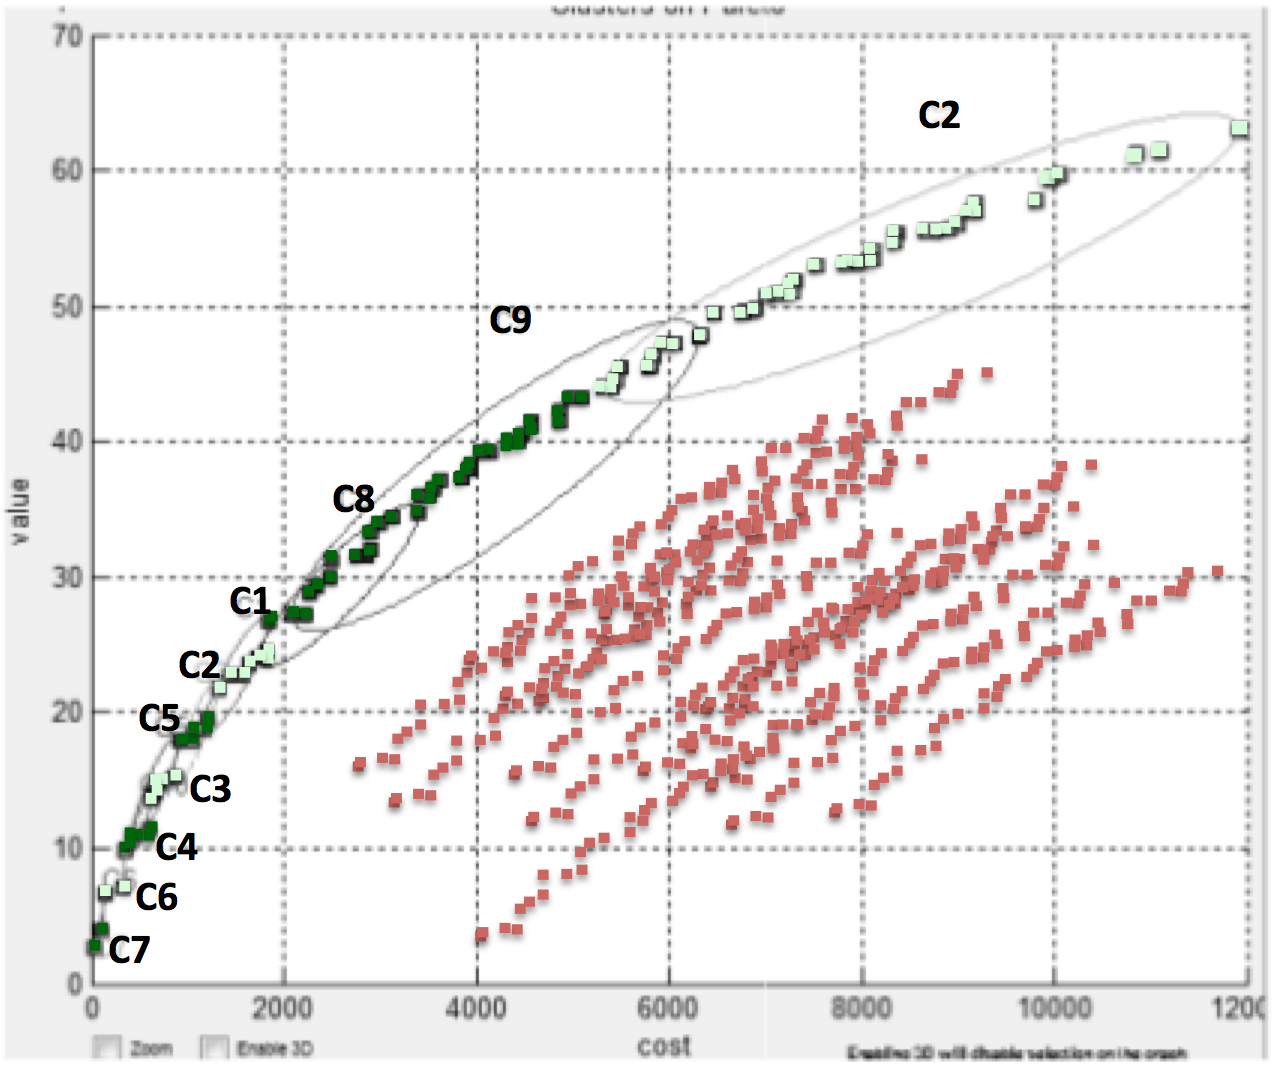
\includegraphics[width=3.5in]{figures/amus.png}
%% \caption{Exploring options for configuring London
%% Ambulances~\cite{veer11} (to minimize $X$ and maximize $Y$).
%% Thousands of options, shown in red, have been rejected
%% to isolate clusters of better solutions C1,C2,etc. }\label{fig:one}
%% \end{figure}

\ADD{One way to simplify the task of understanding these
algorithms is to focus on the {\em Pareto frontier}}; i.e.
the subset of solutions 
that are not worse than any other (across all goals)
but better on at least one goal. 
%% For example,
%% the green dots
%% in \fig{one} are an example of such a Pareto
%% frontier (and the red dots are called the {\em dominated} examples).
The problem here is that even the Pareto frontier can be too large to understand.
Harman cautions that many frontiers are very {\em crowded}; i.e. contain thousands (or more)
candidate solutions~\cite{harm13}.
Hence, researchers like Verrappa and Letier add post-processors
that (a)~cluster the Pareto frontier and
then (b)~show users a small number of examples per cluster. 

That approach has the drawback that
before the users can get their explanation,
some other process must generate the Pareto frontier-- which can be a
very slow computation.  Zuluaga et
al. comment on the cost of such an analysis for
software/hardware co-design: ``synthesis of only one
design can take hours or even
days.''~\cite{Zuluaga:13}.  Harman~\cite{harm13}
comments on the problems of evolving a test suite
for software if every candidate solution requires a
time-consuming execution of the entire system: such
test suite generation can take weeks of execution
time. 

For such slow computational problems, it
would be useful to reason about a problem
using a very small number of most informative
examples. This paper introduces GALE, 
an optimizer that 
identifies and evaluates just those
most informative
examples, as follows:
\begin{changed}
\be
\item Sort solutions (along the direction of most change);
\item Find the {\em poles}; i.e. the two most distance candidates;
\item Split that sort into equal halves;
\item Evaluate only the {\em poles} of each split;
\item Ignore any half containing a dominated pole;
\item Recurse on the remaining halves until the splits get too small (less than $\sqrt{N}$);
\item For all the final (smallest) splits,
  mutate the candidates towards the better pole of
  that split. 
\item Go to step \#1 \ee 
\end{changed}
\noindent
Note that  this a different approach
of Verrappa \& Letier:
GALE does not use clustering as a post-process to some other optimizer.
Rather, GALE {\em replaces} the need for a post-processor with its tool called WHERE, which explores only two evaluations per recursive split
of the data. Hence, this algorithm
performs at most $2{\log_2}(N)$ evaluations per
generation (and even less when step \#5 ignores half of a split).

This paper introduces GALE and its algorithms and 
answers two key research questions.
\begin{quote}
{\bf RQ1 (speed):} Does GALE terminate faster than other multi-goal optimization tools?
\end{quote}
This is a concern since GALE
must  repeatedly sort and divide  the examples (see step \#1, above)--
which might  make  GALE  slower than other multi-goal optimizers.

A second 
concern  is the quality of GALE's results:
\begin{quote}
{\bf RQ2 (quality):} Does GALE return similar or better
solutions than other optimization tools?
\end{quote}
This is a concern since GALE only examines $2\log_2(N)$ of the solutions--
which might mean that GALE misses  useful optimizations
 found by other tools.




The rest of this paper addresses these  research questions.
After  notes on related work (in Section 2)
we present the  details of GALE (in Section 3). 
The algorithm is  tested on many models of varying sizes, using
a range of models described (in Section 4).
Lastly, Section~5 presents answers to the research questions.

As to {\bf RQ1 (speed)}, GALE ran much faster than
other tools, especially for very large models.
For example, 
in our largest model, GALE terminated in four minutes
while other tools needed seven hours.
\begin{changed}
As to {\bf RQ2 (quality)}, we find that
(as might be expected)
GALE's truncated search sometimes explores a smaller  {\em hypervolume}  of 
solutions than other optimizers.
Yet within that smaller volume,   GALE's careful directed search
is more {\em spread} out. More importantly, on inspection of  the raw objective scores,
we often find better results with GALE than with other optimizers. 

From the above, the overall conclusion of this work is:
\begin{quote} {\em
A careful directed search over a small space can find better solutions (with fewer
evaluations)
than a random stagger around a larger volume.}
\end{quote}

\end{changed}


\subsection{Availability}\label{sec:avail}

GALE is released under the GNU Lesser GPL and is available
as part of the JMOO package (Joe's multi-objective optimization), which
incorporates DEAP (Distributed Evolutionary Algorithms in Python~\cite{jmlr12}).
GALE and most of the models used here are available 
from \url{github.com/tanzairatier/jmoo} (and for the XOMO software process model, see
\url{github.com/nave91/modeller/tree/master/xomo}).


%% Lastly, even when humans are not in the loop for reasoning about a model, it is important for search-based
%% SE to reduce the number of evalxfwuations required for controlling a model. As software systems grow ever larger
%% and more complex, it becomes harder to explore all their internal effects. Hence, tools like GALE are required
%% to map out and better understand  the shape of those internal effects.


\begin{changed}
\subsection{Some Frequently Asked Questions}\label{sec:faq} 

{\em Question1: What does all this have to do with Software Engineering?}
In  traditional manual software engineering, engineers laboriously
convert (by hand)
non-executable paper models into executable code. That traditional process
has been the focus of much research.  

This paper is about a new kind of SE which relies, at least in
part, on executable models. In this approach, engineers codify the current
understanding of the domain into a model, and then study those models.

Many of these models are delivered as part of working systems.
So much so that these models now
  mediate nearly all aspects of our lives:
\bi
\item If you
  live in London or New York and need to call an
  ambulance, that ambulance is waiting for your call
  at a location pre-determined by a model~\cite{veer11}. 
\item
If you cross from Mexico to     Arizona,
a biometrics model  decides if you need
secondary screening~\cite{Sacanamboy09}.
\item
 The power to make your toast comes from a
  generator that was spun-up in response
  to some model predicting your future electrical
  demands~\cite{808235}.  
\item
If you fly a plane, extensive
  model-based software controls many aspects of
  flight, including what to do in emergency
  situations~\cite{Kim2011}. \item
If you have a heart attack, the
   models in the defibrillator will
  decide how to shock your heart and lungs so that
  you might live a little longer~\cite{kamp99}.
\ei
We assert that more and more it will be role
of software engineers to build and maintain those models.
Software engineering is a resource-bound activity
so the software engineers responsible
 for model-based software will
need tools like GALE to rapidly build and understand those models
(for examples of the kinds of models that might be processed,
see later in this paper).


{\em Question2: Will GALE work for all models?}
Wolpert and Macready~\cite{wolpert97} showed in 1997
that no optimizers necessarily work better than any
other for all possible optimization
problems\footnote{``The computational
  cost of finding a solution, averaged over all
  problems in the class, is the same for any
  solution method.  No solution therefore offers a
  short cut.''~\cite{wolpert97}}. Hence, when this paper claims that
GALE works comparatively well, we  stress that this conclusion 
is based on the study that applies a few optimizers to the
22 models explored by GALE in Krall's Ph.D. thesis~\cite{krall14f}
and the 43 models explored later in this paper.
That said, GALE is a stand-out result in that we know of no other search-based
SE paper that can achieve GALE's results using so few evaluations.


{\em Question3: does GALE make the (overly simplistic) assumption
that the shape of the Pareto frontier is linear?}  If so, then GALE will
only work on very simple problems.
In reply to this concern, we note that GALE
recursively bisects the solutions into progressively
smaller regions using the spectral learning methods 
discussed in \tion{spectral}. Spectral learners
reflect over the eigenvectors of the data.
These vectors are a model of the overall direction of the
data.  Hence, GALE's splits are not some naive division based
on the raw dimensions. Rather, GALE's splits are very informed about the overall
shape of the data.
GALE's recursive splitting generates a set of
tiny clusters. Each cluster   represents a small space
on the Pareto frontier.  That is, GALE does not
assume that the whole Pareto frontier can be modeled
as one straight line. Rather, it assumes that the
Pareto frontier can be approximated by a set of very
small {\em locally linear} models.

\end{changed}

\newcommand{\Yes}{\ding{51}}
\newcommand{\No}{\ding{55}}


%\begin{figure}[!b]
%\color{MyDarkBlue}
%\b%% egin{center}%35
%% \scriptsize
%% \begin{tabular}{r@{~}|c@{~}|r@{~}|c}
%%      &                     &        Runtime,sec: avg of 100 &            \\
%%      &      Constrained    &   runs, random inputs           &      Ref      \\ \hline
%% BNH : d2-o2       &       \Yes     &       0.01    &       \cite{Binh97mobes:a}    \\      
%% Viennet3 : d2-o3  &       \No      &       0.01    &       \cite{viennetmodels}    \\      
%% Viennet2 : d2-o3  &       \No      &       0.01    &       \cite{viennetmodels}    \\      
%% Viennet4 : d2-o3  &       \No      &       0.01    &       \cite{viennetmodels}    \\      
%% TwoBarTruss : d3-o2       &       \Yes     &       0.01    &       \cite{Chafekar03constrainedmultiobjective}      \\      
%% Golinski : d7-o2  &       \No      &       0.01    &       \cite{golinskimodel}    \\      
%% Water : d3-o5     &       \Yes     &       0.02    &       \cite{watermodel}       \\      
%% ZDT6 : d10-o2     &       \No      &       0.02    &       \cite{Zitzler2000zdtpaper}      \\      
%% DTLZ1 : d5-o2     &       \No      &       0.02    &       \cite{dtlz2001a}        \\      
%% Srinivas : d2-o2  &       \Yes     &       0.03    &       \cite{DBLP:journals/ec/SrinivasD94}     \\      
%% ZDT4 : d10-o2     &       \No      &       0.03    &       \cite{Zitzler2000zdtpaper}      \\      
%% DTLZ5 : d10-o2    &       \No      &       0.03    &       \cite{dtlz2001a}        \\      
%% DTLZ2 : d10-o2    &       \No      &       0.03    &       \cite{dtlz2001a}        \\      
%% DTLZ3 : d10-o2    &       \No      &       0.03    &       \cite{dtlz2001a}        \\      
%% DTLZ4 : d10-o2    &       \No      &       0.03    &       \cite{dtlz2001a}        \\      
%% DTLZ2 : d10-o4    &       \No      &       0.03    &       \cite{dtlz2001a}        \\      
%% DTLZ1 : d5-o4     &       \No      &       0.04    &       \cite{dtlz2001a}        \\      
%% DTLZ4 : d10-o4    &       \No      &       0.04    &       \cite{dtlz2001a}        \\      
%% DTLZ3 : d10-o4    &       \No      &       0.04    &       \cite{dtlz2001a}        \\      
%% DTLZ5 : d10-o4    &       \No      &       0.04    &       \cite{dtlz2001a}        \\      
%% ZDT3 : d30-o2     &       \No      &       0.05    &       \cite{Zitzler2000zdtpaper}      \\      
%% ZDT1 : d30-o2     &       \No      &       0.05    &       \cite{Zitzler2000zdtpaper}      \\      
%% DTLZ6 : d20-o4    &       \No      &       0.05    &       \cite{dtlz2001a}        \\      
%% ZDT2 : d30-o2     &       \No      &       0.06    &       \cite{Zitzler2000zdtpaper}      \\      
%% DTLZ6 : d20-o2    &       \No      &       0.06    &       \cite{dtlz2001a}        \\      
%% Osyczka2 : d6-o2  &       \Yes     &       0.29    &       \cite{osymodel}         \\      
%% Tanaka : d2-o2    &       \Yes     &       0.35    &       \cite{537993}   \\      
%% xomogr : d27-o4   &       \No      &       0.96    &        \cite{me07f,me09a,me09e}       \\      
%% xomofl : d27-o4   &       \No      &       0.96    &         \cite{me07f,me09a,me09e}      \\      
%% xomoo2 : d27-o4   &       \No      &       0.99    &        \cite{me07f,me09a,me09e}       \\      
%% POM3B : d9-o4     &       \No      &       6.28    &       \cite{port08,me09j}     \\      
%% POM3A : d9-o4     &       \No      &       218.98  &       \cite{port08,me09j}     \\      
%% POM3C : d9-o4     &       \No      &       445.03  &       \cite{port08,me09j}     \\      
%% CDA     &       \No      &       8100.00    &       \cite{Kim2011,Pritchett2011,Feigh2012,Kim2013,Pritchett2013}   
%% \end{tabular}           
%% \end{center}
%% \caption{The 35 models used in this study. These come  from the 13 different references shown in the right-hand-side column.
%% The model name is specified in the following format:  \emph{name} - \emph{number of inputs} - \emph{number of objectives}.  For example, ``ZDT3 : d30-o2'' means ZDT3 with 30 decision inputs and 2 objective outputs.
%% For more details on these models, see \tion{models}.}\label{fig:35models}
%% \end{figure} 


\section{Related Work}
This section explains the following terms.
GALE is an {\em active learner} that implements a {\em decomposition-based} {\em multi-objective evolutionary algorithm} (MOEA).
GALE's mutators use  {\em continuous domination} and {\em spectral learning}
to push solutions away from worse regions.

%% \subsection{SBSE}


%% In software engineering (SE), it is often necessary to trade
%% off between many competing objectives.  This task is often handled
%% by search-based software engineering (SBSE) tools.
%% For example, Rodriguez et
%% al.~\cite{rod11} used a systems model of a software project~\cite{deb00afast}
%%  to search for inputs that generate favorable outputs---in this case, outputs that
%% most decrease time and cost while increasing productivity. That study
%% generated a three-dimensional surface model where managers could explore
%% trade-offs between the objectives of cost, timlooke and productivity.  In other
%% work, Heaven \& Letier~\cite{heaven11} studied a quantitative
%% goal graph model of the requirements of the London Ambulance
%% Services. The upper layers of that requirements model were a standard
%% Van Lamsweerde goal graph~\cite{lam00}, while the leaves drew their
%% values from statistical distributions. Using that model, they found
%% decisions that balance speed \& accuracy of ambulance-allocation
%% decisions. Subsequent work by Veerappa \& Letier (discussed in the introduction)
%% explored methods to better explain the generated set of solutions~\cite{veer11}.
%% For a list of other SBSE applications, see \fig{tasks}.

%In software engineering (SE), it is often necessary to trade
%% off between many competing objectives.  This task is often handled
%% by search-based software engineering (SBSE) tools.
%% Due to the complexity
%% of these tasks, exact optimization methods may be impractical.
%% Hence, researchers often resort to various meta-heuristic  approaches.
%% In the 1950s, when
%% computer RAM was very small, a standard technique was simulated
%% annealing (SA)~\cite{kirkpatrick83}. SA generates {\em new} solutions
%% by randomly perturbing (a.k.a. ``mutating'') some part of an {\em old}
%% solution.  {\em New} replaces {\em old} if (a) it scores higher; or
%% (b) it reaches some probability set by a ``temperature'' constant. Initially,
%% temperature is high so SA jumps to sub-optimal solutions (this allows
%% the algorithm to escape from local minima). Subsequently, the
%% ``temperature'' cools and SA only ever moves to better {\em new}
%% solutions.
%% SA is often used in SBSE
%% e.g.~\cite{fea02a,me07f,me07g}, perhaps due to its simplicity.

%% In the 1960s, when more RAM became available, it became standard to
%% generate many {\em new} mutants, and then combine together parts of
%% promising solutions~\cite{goldberg79}.  Such {\em evolutionary
%%   algorithms} (EA) work in {\em generations} over a population of
%% candidate solutions.  Initially, the population is created at random.
%% Subsequently, each generation makes use of select+crossover+mutate
%% operators to pick promising solutions, mix them up in some way, and
%% then slightly adjust them.
%% EAs are also often used in SBSE, particularly in test case generation; e.g.~\cite{andrews07,andrews10}.

%% Later work focused on creative ways to control the
%% mutation process. Tabu search and scatter search
%% work to bias new mutations away from prior
%% mutations~\cite{Glover1986563,Beausoleil2006426,Molina05sspmo:a,4455350}.
%% Differential evolution mutates solutions by
%% interpolating between members of the current
%% population~\cite{storn97}.  Particle swarm
%% optimization randomly mutates multiple solutions
%% (which are called ``particles''), but biases those
%% mutations towards the best solution seen by one
%% particle and/or by the neighborhood around that
%% particle~\cite{pan08}.
%% These methods are often used for parameter tuning for other learners.
%% For example, Cora et al.~\cite{cora10} use tabu search to learn the parameters
%% of a radial bias support vector machine for learning effort estimation models.

%% \begin{figure}[!t]
%% \small
%% \begin{tabular}{|p{3.1in}|}\hline
%% \bi
%% \item
%% {\em  Next release planning:}
%% Deliver most functionality
%% in least time and cost~\cite{zhang07a,bagnall01,DurilloZAHN11}.
%% \item {\em Risk management:} Maximize the covered requirements while minimizing the
%% cost of  mitigations applied  (to avoid possible problems)~\cite{fea02a,feather03,me08b}.
%% \item {\em Explore high-level designs:} Use most features
%% avoiding defects, with  least development time,  avoiding violations of
%% constraints~\cite{sayyad13a,sayyad13b}.
%% \item {\em Improve low-level designs:}
%% Apply automatic refactoring tools to object-oriented design in order improve the internal
%% cohesiveness of that design~\cite{ocinneide12}.
%% \item
%% {\em  Test case generation:} Adjust  test suites
%% to increase program  coverage by those tests~\cite{andrews07,andrews10,me09m}.
%% \item
%% {\em Regression tests:} Find tests that run fastest, with the most odds of being relevant
%% to  recently changed code, with the greatest probability of failing~\cite{weimer13}.
%% \item
%% {\em Cloud computing:}
%% For distributed CPUs and disks, adjust allocation and assignment of tasks
%% to  trade-off between availability,
%% performance and cost~\cite{harman13}.
%% \item
%% {\em Predictive Modeling:} Tune  data miner's parameters to improve  predictions of
%% software cost~\cite{cora10}.
%% \ei\\\hline
%% \end{tabular}
%% \caption{Some optimization tasks explored by SBSE.}\label{fig:tasks}
%% \end{figure}

\subsection{MOEA}\label{sec:w}
Evolutionary optimizers explore {\em populations} of candidate solutions.
In each {\em generation} some {\em mutator} makes changes
to the current population. A {\em select} operator then picks the best mutants
which are then {\em combined} is some manner to become generation $i+1$.
This century, there has been much new work on
multi-objective evolutionary algorithms (MOEA) with 2 or 3 objectives
(as
well as many-objective optimization, with many more
objectives).   
MOEAs address a major drawback with traditional single goal
optimization.

\begin{changed}
In the traditional approach, the space of solution options
was explored by assigning
``magic'' weights to the objectives, then using an {\em aggregation function} to accumulate
the results. Such solutions may be  ``brittle'';
i.e. they
change dramatically if we alter the magic weights.  

To avoid the problem
of magic weights, a multi-objective optimizer tries to produce the space of solutions
that would be generated across all possible values of the magic weights.
Multi-objective evolutionary algorithms
such as NSGA-II, SPEA2, IBEA, PSO, DE, MOEA/D, etc~\cite{deb00afast,zit02,Zitzler04indicator-basedselection,Poli07particleswarm,585892,zhang07},
try to push
a cloud of solutions towards an outer envelope of
preferred solutions.
These algorithms eschew the idea of
single solutions, preferring instead to use the {\em domination function} (discussed below) to
map out the
terrain of all useful solutions.
\end{changed}
 
\begin{changed}
\subsection{Search-based SE = MOEA + SE}\label{sec:abutsbse}
Recently, there has been much interest in applying
MOEAs to many areas of software engineering
including requirements engineering, test case
planning, software process planning, etc. 
This {\em search-based software engineering} is a  rapidly expanding area of research and a full survey of that work is beyond
the scope of this paper (for extensive notes on this topic, see~\cite{harman12abc,harman14}). 
Harman et
al.~\cite{harman12abc} comment  that the popularity of
such SBSE methods comes from core
properties of software:
\begin{quote}
``{\ldots}the virtual nature of
software makes it well suited for (search-based
optimization). The field of SE is imbued with rich
metrics that can be useful initial candidates for
fitness functions{\ldots}(where) fitness is computed
directly in terms of the engineering artifact,
without the need for the simulation and modeling
inherent in all {\em other approaches}.''
\end{quote}
By  ``other approaches'',
Harman et al. refer to optimizers
that demand detailed knowledge  about  the internals
 of a system. For example,
gradient descent optimizers~\cite{saltelli00} require that
models contain only differential functions
(i.e. functions of real-valued variables whose
derivative exists at each point in its
domain).
This is impractical  for  software systems since, often,
they manipulate symbols as well as numbers.
Also the  internal state space of software is
usually not a smoothly differential continuous function.
Rather, software contains many regions
with many different properties (each ``if''
statement in a software system can divide the
internal state space of a program into multiple
regions, each of which can have very different
properties~\cite{lowrey98}).

Another reason to prefer this ``black box'' MOEA approach is that
often we may know  very little about the internal details of software.
Ever since Parnas' 1972 paper ``On the Criteria To
Be Used in Decomposing Systems into
Modules''~\cite{parnas72}, software engineers have
designed their systems as ``modules'' where software's
internal details are ``hidden'' within interface
boundaries.  
This concept of modularity is one of the cornerstones of modern
software engineering since, in such modular systems
(1)~engineers are free
to fix and enhance the internal details of software just as long as they
maintain the same interface;
(2)~engineers can use the services of other systems by connecting to its interface {\em without}
needing to understand the internal details.

Hence, the classic software MOEA 
problem contains:\be
\item
 A system that executes, but we may not fully understand all its internal details;
\item
Inputs represented as a flat vector of decisions;
\item And (1+2) together can 
generate many outputs, which can be assessed by a
fitness function.
\ee
GALE was designed to support this
classic MOEA problem-- with one additional requirement
discussed in the introduction (some systems are too
slow to allow too many evaluations; if users are to certify the correctness of the conclusions, then
we need to present them with a very limited number of example for their inspection):
\begin{enumerate}
\setcounter{enumi}{3}
\item Optimization needs very few system evaluations.
\end{enumerate}
As an aside, we note that elsewhere, we have applied MOEA to other kinds of software systems that make changes
to some of the above assumptions. For example, Sayyad, Menzies et al.~\cite{sayyad13a,sayyad13b} 
adapted
MOEA to systems containing hierarchical  constraints, for which we
have  100\% knowledge of the internal structure.
In that work, that structural knowledge was exploited via {\em push} and {\em pull} strategies
that use decisions made in
one part of a system to reduce the search space in
other parts of the same system. Note that for the ``black box'' systems described in classic
software MOEA problem, such {\em push,pull} strategies cannot be applied (since the internal
structure of the software is unknown).
\end{changed}
\subsection{MOEA and Domination}\label{sec:cdom}


To explore the space of promising solutions,
MOEA tools
use a
{\em  domination function} to
find
promising solutions for use in the next generation. 
Domination functions have the property
that, when they compare candidate solutions with many competing objectives,
they accept large sets (and not just single items) as being better than others.
Hence, they are candidate techniques for generating the space of possible solutions.


{\em Binary domination} says that solution $x$ ``dominates''
solution $y$ if solution $x$'s objectives are never worse than  solution $y$
and at least one objective in solution $x$ is better than its counterpart in $y$; i.e.
 $\left\{ \forall o  \in \textit{objectives}\;\mid\; \neg ( x_o \prec y_o )\right\}$
and
 $\left\{
\exists o \in \text{objectives} \;\mid\; x_o \succ y_o\right\}$, where ($\prec,\succ$) tests if $x_o$ is (worse,better) than $y_o$.
 Recently, Sayyad~\cite{sayyad13a} studied binary domination for MOEA
with 2,3,4 or 5 objectives.  Binary domination performed as well as anything else
for 2-objective problems but very few good solutions were found for
the 3,4,5-goal problems.  The reason was simple: binary domination  only returns
{\em \{true,false\}}, no matter the difference between $x_1,x_2$. As the objective
space gets more divided at higher dimensionality, a more nuanced approach is required.


While binary domination just returns (true,false), a {\em continuous domination} function sums
the total improvement of solution $x$ over all other solutions~\cite{Zitzler04indicator-basedselection}.
In the IBEA genetic algorithm~\cite{Zitzler04indicator-basedselection}, continuous domination is defined as the sum of the
differences between objectives (here ``$o$'' denotes the number of objectives),
raised to some exponential power.
Continuous domination favors $y$ over $x$ if $x$ ``losses'' least:

\begin{equation}\label{eq:cdom}
\begin{array}{rcl}
\textit{worse}(x,y)& =& \textit{loss}(x,y) > \textit{loss}(y,x)\\
\textit{loss}(x,y)& = &\sum_j^o -e^{w_j(x_j - y_j)/o	} / o
\end{array}
\end{equation}
In the above, $w_j\in \{-1,1\}$, depending on whether
we seek to maximize goal $x_J$.   
To prevent issues with exponential functions,
the objectives are normalized.

\lstset{
    language=Python,
    basicstyle=\ttfamily\fontsize{2.7mm}{0.8em}\selectfont,
    breaklines=true,
    prebreak=\raisebox{0ex}[0ex][0ex]{\ensuremath{\hookleftarrow}},
    frame=l,
    showtabs=false,
    showspaces=false,
    showstringspaces=false,
    keywordstyle=\bfseries,
    emph={furthest,gale,better,improved,where,fastmap,split,project,mutate,mutate1}, emphstyle=\bfseries\color{blue},
    stringstyle=\color{green!50!black},
    commentstyle=\color{gray}\itshape,
    numbers=left,
    captionpos=t,
    escapeinside={\%*}{*)}
}

\subsection{MOEA Algorithms}\label{sec:algo}
A standard
MOEA strategy is to generate new individuals, and then
focus just on those on the Pareto
frontier. 
For example, 
 NSGA-II~\cite{deb00afast} 
uses a non-dominating sort
procedure to divide the solutions into {\em bands}
where {\em band}$_i$ dominates all of the solutions
in {\em band}$_{j>i}$ (and NSGA-II favors the
least-crowded solutions in the better bands).

\begin{changed}

There are other kinds of MOEA algorithms including the following
(the following list is not
exhaustive since, to say the least,   this is a very
active area of research):
\bi
\item
{\em SPEA2}: favors solutions
that dominate the most number of other solutions
that are not nearby (to break ties, it uses 
density sampling)~\cite{zit02}; 
\item {\em  IBEA}:
uses continuous dominance to find the solutions
that dominate all others~\cite{Zitzler04indicator-basedselection}; 
\item In {\em Particle swarm
  optimization}, a ``particle'''s velocity is 
``pulled' towards the individual and the community's
best current solution~\cite{pan08,V.Sedenka2010,Kennedy:2001:SI:370449,Poli07particleswarm};
\item 
The {\em many-objective
optimizers}  designed for very high
numbers of objectives~\cite{deb14}; 
\item
Multi-objective {\em
differential evolution}: members of
the frontier compete (and are possibly replaced) by
candidates generated via extrapolation among  any three
other members of the frontier~\cite{storn97,5601760};
\item
The {\em decomposition methods} discussed below.
\ei 


\subsection{MOEA and Decomposition}\label{sec:decomp}

Another way to explore solutions is to
apply some heuristic to decompose the total
space into many smaller problems, and then use a simpler
optimizer for each region. For example, in
$\mathcal{E}$-domination~\cite{deb05}, each objective $o_i$ is
divided into equal size boxes of size $\mathcal{E}_i$
(determined by asking users ``what is their lower
threshold on the size of a useful effect?'').  Each
box has a set $X.\mathit{lower}$ containing boxes
with worse $o_i$ values.  Solutions in the same box are
assessed and pruned in the usual way (all-pairs computation
of a dominance function). But solutions in different
boxes can be quickly pruned via computing dominance
for small samples from each box. Once a box $X$ is
marked ``dominated'', then $\mathcal{E}$-domination 
uses the boxes
like a reverse index to 
quickly find all solutions in $X.\mathit{lower}$, then
mark them as ``dominated''.

Later research generalized this approach.
MOEA/D (multiobjective
evolutionary algorithm based on
decomposition~\cite{zhang07}) is a generic framework
that decomposes a multiobjective optimization
problem into many smaller single problems, then
applies a second optimizer to each smaller subproblem,
simultaneously. 

GALE uses MOEA decomposition but avoids certain 
open issues with   $\mathcal{E}$-domination and MOEA/D. 
GALE does not need some outside oracle to specify
$\mathcal{E}$. Rather, the size of the subproblems is determined
via a recursive median split
on dimensions synthesized
using a PCA-approximation algorithm-- see the  {\em fast spectral learning}
described in the next section. Also, GALE does not need MOEA/D's secondary optimizer to handle 
the smaller subproblems. Rather, our approach uses  the synthesized dimensions
to define the {\em geometry-based mutator}
discussed below
that ``nudges'' all candidates in a subproblem towards the better half of that subproblem. 

\end{changed}



When domination is applied to a
population it can be used to generate the {\em
  Pareto frontier}, i.e.  the space of non-dominated
and, hence, most-preferred solutions.  However, if applied without care,
the number of evaluations of candidate solutions can accumulate.  The goal of GALE
is to minimize this number of evaluations, via applying the {\em fast spectral learning}
and {\em active learning} techniques discussed in the next two sections.




%% \begin{figure}[!t]
%% {\fontsize{2mm}{0em}\selectfont 
%% ~~~~~~~~\begin{minipage}[t]{1.5in}
%% {\small 
%% {\bf Figure4a:} 
%% Dividing 400 instances using just the independent variables.}

%% \begin{verbatim}
%% 400
%% |  > 200
%% |  |  > 100
%% |  |  |  > 50
%% |  |  |  |  > 25
%% |  |  |  |  < 25
%% |  |  |  < 50
%% |  |  |  |  > 25
%% |  |  |  |  < 25
%% |  |  < 100
%% |  |  |  > 50
%% |  |  |  |  > 25
%% |  |  |  |  < 25
%% |  |  |  < 50
%% |  |  |  |  > 25
%% |  |  |  |  < 25
%% |  < 200
%% |  |  > 100
%% |  |  |  > 50
%% |  |  |  |  > 25
%% |  |  |  |  < 25
%% |  |  |  < 50
%% |  |  |  |  > 25
%% |  |  |  |  < 25
%% |  |  < 100
%% |  |  |  > 50
%% |  |  |  |  > 25
%% |  |  |  |  < 25
%% |  |  |  < 50
%% |  |  |  |  > 25
%% |  |  |  |  < 25
%% \end{verbatim}
%% \end{minipage}~~~~~~~~~\begin{minipage}[t]{1.5in}
%% {\small
%% {\bf Figure4b}: Dominated sub-trees are pruned via active learning techniques(~\tion{al}).}

%% \begin{verbatim}
%% 400           
%% |  > 200  <-- pruned
%% |  < 200 
%% |  |  > 100 
%% |  |  |  > 50 <-- pruned
%% |  |  |  < 50 
%% |  |  |  |  > 25 <-- pruned
%% |  |  |  |  < 25 
%% |  |  < 100 
%% |  |  |  > 50 
%% |  |  |  |  > 25 
%% |  |  |  |  < 25 
%% |  |  |  < 50 
%% |  |  |  |  > 25 
%% |  |  |  |  < 25 
%% \end{verbatim}
%% \end{minipage}}
%% \caption{Recursive division via WHERE of 400 instances 
%% (using FastMap).}\label{fig:cluster1}
%% \end{figure}
 


\subsection{Fast Spectral Learning}\label{sec:spectral}
This section describes how GALE
decomposes a large space of candidate solutions into many smaller
regions.

WHERE is a {\em spectral learner}~\cite{KamvarKM03}; i.e. given solutions with $d$ possible decisions,
it
re-expresses those $d$ decision variables in terms of the
$e$ eigenvectors of that data.
This speeds up the reasoning since we then only need to
explore the $e\ll d$   eigenvectors.

A widely-used spectral learner is a principal
 components analysis (PCA).  For example, PDDP ({\em
 Principal Direction Divisive
 Partitioning})~\cite{boley98} recursively
 partitions data according to the median point of
 data projected onto the first PCA component of the
 current partition.

WHERE~\cite{me12d} is a linear time variant of PDDP  that uses FastMap~\cite{Faloutsos1995}
to quickly find the first component.
Platt~\cite{platt05} shows that FastMap is a  Nystr\"om 
algorithm that finds approximations to eigenvectors.
As shown in \fig{fastmapCode} on lines 3,4,5, FastMap  projects all data onto a line
connecting two distant points\footnote{
To define distance, WHERE uses 
the standard Euclidean distance method proposed by 
Aha et al.~\cite{aha91}; that is:
$dist(x,y)= \sqrt{\sum_{i\in d} (x_i - y_i)^2}/\sqrt{ 
\left\vert{d}\right\vert }$ where distance is
computed on the independent decisions $d$ of each candidate solution;
all $d_i$ values are normalized min..max, 0..1; and the calculated distance normalized by dividing by the maximum distance
across the $d$ decisions.}. 
FastMap finds these two distant points in near-linear
time. The search for the poles needs only
$O(N)$ distance comparisons (lines 19 to 24).
The slowest part of this search is the sort used to find the median $x$ value 
(line 10) but even that
can be reduced to  asymptotically optimal linear-time
via the standard median-selection algorithm~\cite{hoare61}.

FastMap returns the data split into two
equal halves.
WHERE recurses on the two halves,
terminating when some split
has less than $\sqrt{N}$ items.


\begin{figure}[!b]
\begin{lstlisting}[mathescape,frame=l,numbers=left]
def fastmap(data): 
  "Project data on a line between 2 distant points"
  z          = random.choose(data)
  east       = furthest(z, data)
  west       = furthest(east, data)
  data.poles = (west,east)
  c          = dist(west,east)     
  for one in data.members: 
    one.pos = project(west,east,c,one)
  data = sorted(data) # sorted by 'pos'
  return split(data)

def project(west, east, c, x): 
  "Project x onto line east to west"
  a = dist(x,west)
  b = dist(x,east)
  return (a*a + c*c - b*b)/(2*c) # cosine rule

def furthest(x,data): # what is furthest from x?
  out, max = x,0
  for y in data:
    d = dist(x,y)
    if d > max: out, max = y, d
  return out

def split(data): # Split at median
   mid = len(data)/2; 
  return data[mid:], data[:mid]
\end{lstlisting}
\caption{Splitting data with FastMap}
\label{fig:fastmapCode}   
\end{figure}

\subsection{Active Learning}

One innovation in GALE is its use of  {\em active learning} during
WHERE's decomposition of larger problems into sub-problems.
Active learners make conclusions by asking for {\em
more} information on the {\em least} number of
items.  For optimization,  such active learners
reflect over a population of decisions and only
compute the objective scores for a small, {\em most
informative subset} of that
population~\cite{Zuluaga:13}. 
GALE's active learner finds its {\em most information subset} via the WHERE
clustering procedure described above.
Recall that
WHERE recursively divides the candidates into many small clusters,
and then looks for two most different (i.e. most distant) points
in each cluster. For each cluster, GALE then evaluates only these
two points. 

In other work, Zuluaga et
al.~\cite{Zuluaga:13} use a {\em response surface
  method} for their MOEA active learner.  Using some
quickly-gathered information, they build an
approximation to the local Pareto frontier using a
set of Gaussian surface models. These models allow
for an extrapolation from \ADD{known members of the
population to new and novel members}.  Using these models, they can then
generate approximations to the objective scores of
mutants. Note that this approach means that (say)
after 100 evaluations, it becomes possible to
quickly approximate the results of (say) 1000 more.


\begin{figure}[!b]
\begin{lstlisting}[mathescape,frame=r,numbers=right]
def where(data, scores={}, lvl=10000, prune=True):  
  "Recursively split data into 2 equal sizes."
  if lvl < 1: 
     return data # stop if out of levels
  leafs      = [] # Empty Set
  left,right = fastmap(data)
  west, east = data.poles
  $\omega=\sqrt{\mu}$ # enough data for recursion
  goWest = len(left) > $\omega$  
  goEast = len(right) > $\omega$ 
  if prune: # if not pruning, ignore this step
    if goEast and better(west,east,scores): 
       goEast = False 
    if goWest and better(east,west,scores): 
       goWest = False 
  if goWest:  
     leafs += where(left,  lvl - 1, prune)  
  if goEast:  
     leafs += where(right, lvl - 1, prune) 
  return leafs

def better(x,y,scores):
   "Check if not worse(y,x) using $\eq{cdom}$. If any"
   "new evaluations, cache them  in 'scores'."
\end{lstlisting}

\caption{Active learning in GALE:
recursive division of the data;
only evaluate two distant points in each cluster;
only recurse into non-dominated halves.
In this code, $\mu$ is size of the original data set.
}
\label{fig:whereCode}   
\end{figure}


\begin{changed}
Unlike Zuluaga et al., GALE makes no Gaussian parametric assumption about regions
on the Pareto frontier.  Rather, it uses a non-parametric approach (see below).

That said, GALE and  Zuluaga et al.  do share one  assumption; i.e that
the Pareto frontier can be approximated by many tiny models.
We defend that assumption as follows. Firstly, it works (see the results, below).
Secondly, 
if this
assumption were wrong, and if there were no similar
properties in local regions, then very small {\em
  and} very large mutations in  evolutionary 
algorithms would be equally effective. Our reading
of the literature is that
standard practice  is to restrain
mutation to just small amounts of just a few attributes~\cite{goldberg00}.
That is, (1)~very large mutations are depreciated; and (2)~GALE's
locality assumption is  generally  endorsed (albeit, implicitly)  by the 
research community.
\end{changed}







\section{Inside GALE}
The  {\em \underline{g}eometric}, {\em \underline{a}ctive \underline{le}arner} called 
GALE interfaces to models using the following functions:
\bi
\item Models create candidates, each  with $d$ decisions. 
\item $\mathit{lo}(i), \mathit{hi}(i)$ report the minimum and maximum
legal values for decision $i\in d$.
\item $\mathit{valid}(\mathit{candidate})$ 
checks if the decisions
do not violate any domain-specific constraints.
\item  From the decisions,
a model can compute $o$  objective scores (used in \eq{cdom}).
\item $\mathit{minimizing}(j)$ returns true,false if the goal
is to minimize,maximize (respectively) objective $j \in o$.
\ei
%% GALE explores the candidates via a combination of optimization and data
%% mining. Given a current population of candidates, the
%% algorithm learns a decision tree whose leaves are non-dominated
%% candidates. These leaves are the seeds for the next generation 
%% of candidates.




\subsection{Active Learning and GALE}\label{sec:al}
GALE's active learner, shown in \fig{whereCode}, is a
variant to the WHERE spectral
learner discussed above.
To understand this procedure, recall 
that WHERE splits the data
into smaller
 clusters, each of which is characterized by two
distant points called {\em west,east}. In that space,
{\em left} and {\em right} are  50\% of the
data, projected onto a line running {\em west} to {\em east},
 split at the median.
When exploring $\mu$ candidates, recursion
halts at splits smaller
than $\omega=\sqrt{\mu}$.


GALE's active learner assumes that it
only needs to evaluate
the 
{\em most informative subset} 
consisting of the {\em poles} used to
recursively divide the data. 
Using \eq{cdom}, GALE checks for domination between
the poles and only recurses into any non-dominated halves.
This process, shown in \fig{whereCode}, uses FastMap
to split the data. 
In  \fig{whereCode}, 
 lines 12 and 14 show the domination
pruning that disables recursion into any dominated half.


Given GALE's recursive binary division of $\mu$ solutions, and that this
 domination tests only two
solutions in each division, then GALE
performs  a maximum of $2log_2(\mu)$ evaluations. Note that when GALE prunes sub-trees,
the actual number of evaluations is less than this maximum.


\subsection{Geometry-based Mutation}\label{sec:geom}
Most MOEAs build their next generation of solutions
by a {\em random mutation} of members of the last
generation. GALE's mutation policy is somewhat
different in that it is a {\em directed mutation}.
Specifically, GALE reflects on the geometry of the
solution space, and mutates instances along
gradients within that geometry. 

To inspect that geometry, GALE reflects over the poles
in each leaf cluster. When one pole
is {\em better} than another, it makes sense to
nudge all solutions in that cluster away from the
worse pole and towards the better pole.
By nudging solutions along a line
running from {\em west} to {\em east}, we are
exploiting spectral learning to implement a {\em
spectral mutator}; i.e. one that works across a
dimension of greatest variance that is synthesized
from the raw dimensions.  That is, GALE models the
local Pareto frontier as many linear models
drawn from the local eigenvectors of different
regions of the solution space. 

\begin{changed}
GALE's mutator is shown in \fig{mutantCode}.
The 
$\Delta$ parameter
is the ``accelerator''
that increases mutation size (in line 20)
while the  $\gamma$ parameter is the ``brake''
that blocks excessive mutation (in line 24).

\end{changed}

\subsection{Top-level Control}

\fig{galeCode} shows GALE's top-level controller.  As seen in that figure, 
the algorithm  is an
evolutionary learner which iteratively builds,
mutates, and prunes a population of size $\mu$
using the active
learning version of WHERE.
The {\em candidates} function (at line 3 and 18) adds random items to the 
population. The first call to this function (at line 3)
adds $\mu$ new items. The subsequent call (at line 18) rebuilds the population back up to $\mu$ after
WHERE has pruned solutions in dominated clusters.

Also shown in that figure is GALE's termination
procedure: GALE exits after $\lambda$ generations with no improvement
in any goal.
Note that, on termination, GALE calls WHERE one last
time at line 15 to find {\em enough} examples to
show the user. In this call, domination pruning is
disabled, so this call returns the poles of the
leaf clusters.


\begin{figure}[!t]
\begin{lstlisting}[mathescape,frame=r,numbers=right]
def mutate(leafs, scores): 
  "Mutate all candidates in all leafs."
  out = [] # Empty Set
  for leaf in leafs:
    west,east = leafs.poles
    if better(west,east, scores): # uses Equation 1
       east,west = west,east # east is the best pole
    c = dist(east,west)
    for candidate in leaf.members:
      out += [mutate1(candidate, c, east, west)]
  return out 

def mutate1(old,c,east,west,$\gamma$=1.5,$\Delta$=1): 
  "Nudge the old towards east, but not too far."
  new    = copy(old)
  for i in range(len(old)):
    d = east[i] - west[i]
    if not d == 0: #there is a gap east to west
      d= -1 if d < 0 else 1 #d is the  direction
      x= $\Delta$*new[i]* (1+ abs(c)*d) #nudge along d 
      new[i]= max(min(hi(i),x),lo(i))#keep in range
  newDist = project(west,east,c,new) -
            project(west,east,c,west)
  if (abs(newDist) < $\gamma$*abs(c)) and valid(new): 
    return new
  else: return old
\end{lstlisting}

\caption{Mutation with GALE.
By line 7, GALE has determined that the {\em east}
pole is preferred  to {\em west}.
At line 23,24, the {\tt project}
function of \fig{fastmapCode}  is used
to check 
we are not rashly mutating a candidate too far away from
the region that originally contained it.}
\label{fig:mutantCode}   
\end{figure}
\begin{figure}[!t]
\begin{lstlisting}[mathescape,frame=r,numbers=right]
def gale(enough=16,  max=1000,  $\lambda=3$):
  "Optimization via Geometric active learning"
  pop      = candidates($\mu$) # the initial population
  patience = $\lambda$
  for generation in range(max):
    # mutates candidates in non-dominated leafs
    scores  = {} # a cache for the objective scores 
    leafs   = where(pop, scores)
    mutants = mutate(leafs, scores)
    if generation > 0:  
      if not improved(oldScores ,scores):
        patience = patience - 1 #losing  patience
      oldScores = scores #needed for next generation
      if patience < 0: #return enough candidates
        leafs=where(pop,{},log2(enough),prune=False)
        return [ y.poles for y in leafs ] 
    #build up pop for next generation
    pop = mutants + candidates($\mu$-len(mutants))   

def improved(old,new):
  "Report some success if any improvement."
  for j in range(len(old)):
    before = # old mean of the j-th objective
    now    = # new mean of the j-th objective
    if minimizing(j):
      if now < before: return True
    elif now > before: return True
  return False 
\end{lstlisting}

\caption{GALE's top-level driver.}
\label{fig:galeCode}   
\end{figure}




\begin{changed}
\addit{cocont}

\section{Models Used in This Study}\label{sec:models}
Having described general details on MOEA, and the particular details of our approach,
we turn now to the models used to evaluate GALE.
With one exception, all these  are available to other researchers via the websites mentioned in 
\tion{avail}. The exception is the CDA model since that
requires extensive connection to proprietary NASA hardware and software.

The XOMO model~\cite{me07f,me09a,me09e}
combines four software process models from
Boehm’s group at the University of Southern California.
It reports four-objective scores (which we will try to minimize):
project {\em risk};
development {\em effort} and {\em defects}; and total {\em months} of development.

The POM3 model~\cite{port08,me09j}  implements the Boehm and Turner model~\cite{port08,1204376,turner03}
of agile programming
where teams select tasks as they appear in the scrum backlog.
POM3 studies the implications of different ways to adjust task lists in the face of shifting priorities.



The CDA model~\cite{Kim2011,Pritchett2011,Feigh2012,Kim2013,Pritchett2013}
lets an engineer explore the implications of how software presents an airplane's status to a pilot
in safety critical situations.
CDA models how pilots interact with cockpit avionics software
during a continuous descent approach.

Apart from the above three models, we also explore numerous
small maths models that are often used
to benchmark MOEA
problems 
These models are called 
BNH, 
Golinski, 
Srinivas, 
Two-bar Truss, 
Viennet2, 
Water 
ZDT(1,2,3,4 and 6), 
and DTLZ(1,2,3,4,5 and 6).
The  DTLZ suite of models is particularly useful for evaluation of MOEAs since,
by adjusting certain model  parameters, it is possible to generate
problems with a wide range of decisions and objectives~\cite{Zitzler2000zdtpaper,dtlz2001a}.

For more details on these models, see the text below.
For full details on the maths models, see the appendix
(\fig{uncon} and \fig{con} and \fig{dtlzmodels}).





\addit{xomo}

\addit{xomocases}

\end{changed}

\begin{figure*}%[!t]
\scriptsize

  \centering
    \begin{tabular}{|l|l|p{4in}|c|}
        \hline
        Short name &Decision             & Description         &Controllable                                        \\ \hline
        Cult&Culture              & Number (\%) of requirements that change. & yes \\\hline
        Crit&Criticality           & Requirements cost effect for safety critical systems  (see \eq{cmcrit} in the appendix). & yes\\\hline
        Crit.Mod&Criticality Modifier & Number of (\%) teams affected by criticality   (see \eq{cmcrit} in the appendix).   & yes           \\ \hline
        Init. Kn&Initial Known        & Number of (\%) initially known requirements.             & no     \\ \hline
        Inter-D&Inter-Dependency     & Number of (\%) requirements that have interdependencies.  Note that dependencies are requirements within
the {\em same} tree (of requirements), but interdependencies are requirements that live in {\em different} trees.   & no            \\\hline
        Dyna&Dynamism             & Rate of how often new requirements are made (see \eq{dymn} in the appendix). & yes                    \\ \hline
        Size&Size            & Number of base requirements in the project.& no \\        \hline
        Plan&Plan                 & Prioritization Strategy (of requirements): one of
        0= Cost Ascending;  1= Cost Descending; 2= Value Ascending; 3= Value Descending;
        4 = $\frac{Cost}{Value}$ Ascending.
%Note that a standard agile strategies use ``Value Descending'', i.e. plan=3~\cite{me09j}.
 & yes \\\hline
     T.Size&Team Size            & Number of personnel in each team   & yes                         \\ 
        \hline
    \end{tabular}
    \caption {List of Decisions used in POM3. 
The optimization task is to find settings for the controllables in the last column.
}\label{fig:pom3decisions}
\end{figure*}
\begin{figure*}%[!t]
\footnotesize
\begin{center}
    \begin{tabular}{r|p{1.5in}|p{1.5in}|p{1.5in}}
                     & POM3a                         & POM3b             &POM3c       \\ 
                             & A broad space of projects. & Highly critical small projects& Highly dynamic large projects\\\hline
        Culture              & 0.10 $\leq x \leq$ 0.90       & 0.10 $\leq x \leq$ 0.90  & 0.50 $\leq x \leq$ 0.90  \\ 
        Criticality          & 0.82 $\leq x \leq$ 1.26       & 0.82 $\leq x \leq$ 1.26   & 0.82 $\leq x \leq$ 1.26  \\ 
        Criticality Modifier & 0.02 $\leq x \leq$ 0.10       & 0.80 $\leq x \leq$ 0.95 & 0.02 $\leq x \leq$ 0.08   \\ 
        Initial Known        & 0.40 $\leq x \leq$ 0.70       & 0.40 $\leq x \leq$ 0.70  & 0.20 $\leq x \leq$ 0.50  \\ 
        Inter-Dependency     & 0.0   $\leq x \leq$ 1.0       & 0.0   $\leq x \leq$ 1.0  & 0.0   $\leq x \leq$ 50.0 \\ 
        Dynamism             & 1.0   $\leq x \leq$ 50.0      & 1.0   $\leq x \leq$ 50.0  & 40.0   $\leq x \leq$ 50.0 \\ 
        Size                 & x $\in$ [3,10,30,100,300] & x $\in$ [3, 10, 30]     & x $\in$ [30, 100, 300]   \\ 
        Team Size            & 1.0 $\leq x \leq$ 44.0        & 1.0 $\leq x \leq$ 44.0  & 20.0 $\leq x \leq$ 44.0    \\ 
        Plan                 & 0 $\leq x \leq$ 4             & 0 $\leq x \leq$ 4    & 0 $\leq x \leq$ 4       
\end{tabular}
\end{center}

\caption{Three classes of projects studied using POM3. }\label{fig:POM3abcd}
\end{figure*}




\subsection{POM3: A Model of Agile Development}\label{sec:pom3pom3}
POM is short for \underline{P}ort,
\underline{O}lkov and \underline{M}enzies, and is an
implementation of the Boehm and Turner model of
agile programming. For further
details on this model 
see~\cite{port08,1204376,turner03} but, in brief, in agile development, 
teams adjust
their task list according to shifting priorities.

\begin{changed}
Turner and Boehm say that the agile
management challenge is to strike a balance between {\em idle rates},
{\em completion rates} and {\em overall cost}. 
\bi
\item
In the agile world, projects terminate after achieving a 
{\em completion rate} of   $(X<100)$\% of its required tasks.
\item
Team members  become
{\em idle} if forced to wait for a yet-to-be-finished task from other teams. 
\item
To lower {\em idle rate} and  
increase {\em completion rate}, management can hire staff- but this
increases  {\em overall cost}.
\ei
\end{changed}
\fig{pom3decisions}  list some of POM3's variables.
These inputs
characterize the difference
between plan-based and agile-based methods:
\bi
\item {\em Tsize}: project size
\item {\em Crit:} project criticality. In Boehm \& Turner's model
 {\em more} critical projects cost exponentially {\em more} 
according to the formula: $\textit{cost} = \textit{cost} * {C_M}^{\textit{crit}}$.
\item {\em Crit Mod:} the criticality modifier $C_m$ term.
\item {\em Dyna:} dynamism: changes to priorities, costs.
\item {\em Personnel}: the developer skill-level.
\item  {\em Cult:} organizational culture. The {\em larger} this number, the {\em more} conservative
the team and the {\em less} willing to adjust the priority of a current task-in-progress.
\ei
POM3 uses the following parameters to define a space of options.
\bi
\item {\em Size:} number of requirements.
\item {\em Init Kn:} percent of requirements that are initially visible to the team.
\item {\em Plan:} the planning method used to select the next requirement to implement.
\item {\em Inter-D:}  the percent of requirements that have inter-dependencies 
between requirements in other trees.
\ei

  Within this model, POM3 represents requirements as a set of trees.  
    Each tree of the requirements
    heap represents a group of requirements wherein a single node of the
    tree represents a single requirement.  A single requirement consists
    of a prioritization value and a cost, along with a list of
    child-requirements and dependencies.  Before any requirement can be
    satisfied, its children and dependencies must first be satisfied.
    
   POM3 builds a requirements heap with prioritization values,
    containing
     30 to 500 requirements, with costs from 1 to 100 (values 
     chosen in consultation with Richard Turner).  Initially,
    some percent of the requirements are marked
    as visible, leaving the rest to be revealed as teams work on the
    project.

The task of completing a project's requirements is divided amongst teams
    relative to the size of the team (by ``size'' of team, we refer to
    the number of personnel in the team).  In POM3, team size is a decision
    input and is kept constant throughout the simulation.  As a further
    point of detail, the personnel within a team fall into one of three
    categories of programmers: Alpha, Beta and Gamma.  Alpha programmers
    are generally the best, most-paid type of programmers while Gamma
    Programmers are the least experienced, least-paid.  The ratio of personnel type
    follows the Personnel decision as set out by Boehm and Turner\cite{1204376} in the following table:    
    \[\scriptsize
    \begin{array}{l|l|l|l|l|l}
             \multicolumn{1}{c}{~}   & \multicolumn{5}{c}{\textit{project size}}\\\cline{2-6}
                & 0    & 1    & 2    & 3    & 4    \\ \hline
            \textit{Alpha} & 45\% & 50\% & 55\% & 60\% & 65\% \\ 
            \textit{Beta}  & 40\% & 30\% & 20\% & 10\% & 0\%  \\ 
            \textit{Gamma} & 15\% & 20\% & 25\% & 30\% & 35\% \\ 
        \end{array}
    \]
    After teams are generated and assigned to requirements, costs are
    further updated according to decision for the Criticality and
    Criticality Modifier.  Criticality affects the
    cost-affecting nature of the project being safety-critical, while the
    criticality modifier indicates a percentage of teams affected by
    safety-critical requirements.  In the formula, $C_M$ is the {\em criticality
    modifier}:
    \begin{equation}\label{eq:cmcrit}
    \textit{cost} = \textit{cost} * {C_M}^{\textit{criticality}}
    \end{equation}
    
After generating the
    Requirements \& Teams, POM3 runs through the follow five-part {\em shuffling} 
    process (repeated   \mbox{$1 \le N \le 6$} times, selected
    at random).
    
    {\em 1) Collect Available Requirements.} Each team searches through
    their assigned requirements to find the available, visible
    requirements (i.e. those without any  unsatisfied dependencies
    or unsatisfied child requirements).  At this time, the team budget
    is updated, by calculating the total cost of tasks remaining for the
    team and dividing by the number of shuffling iterations:
    \[\textit{team.budget} = \textit{team.budget} + \textit{totalCost/numShuffles}\]
    
    {\em 2) Apply a Requirements Prioritization Strategy.}  After the
    available requirements are collected, they are then sorted per some
    sorting strategy. In this manner, requirements with higher priority
    are to be satisfied first. To implement this, the requirement's cost
    and value are considered along with a strategy, determined by the
    plan decision.
    
    {\em 3) Execute Available Requirements.} The team executes the
    available requirements in order of step2's prioritization.
    Note that some requirements may not get executed due to budget allocations.
    
    {\em 4) Discover New Requirements.} As projects mature, sometimes new requirements are discovered.  To model the probability of new requirement arrivals, the input decision called Dynamism is used in a Poisson distribution.  
    The following formula  is used to add to the percentage of known requirements in the heap:
    \begin{equation}\label{eq:dymn}
    \textit{new} = \textit{Poisson}\left(\textit{dynamism}/10\right)
    \end{equation}
    {\em 5) Adjust Priorities.} In this step, teams adjust their priorities by making use of the Culture $C$ and Dynamism 
    $D$ decisions.  Requirement values are adjusted per the formula along a normal distribution, and scaled by a project’s culture:
    \[
    \textit{value} = \textit{value} + \textit{maxRequirementValue}*\textit{Normal}(0, D)*C
    \]  

When we ran POM3 through various MOEAs, we noticed a strange pattern in the results
(discussed below). To check if that pattern was a function of the model or the MOEAs,
we ran POM3 for the three different kinds of projects shown in \fig{POM3abcd}.
We make no claim that these three classes represent the space of all possible projects.
Rather, we just say that for several kinds of agile projects,
GALE appears to out-perform NSGA-II and SPEA2.

%XXX flip XOMO and POM. make sure pom3abc is mentioned


\subsection{CDA: An Aviation Safety Model}\label{sec:cda}

The CDA continuous descent model is used for the model-based design of cockpit avionics software~\cite{Kim2011,Pritchett2011,Feigh2012,Kim2013,Pritchett2013}.
Internally, CDA
models the physical aerodynamics of an aircraft's flight, the surrounding environment (e.g. winds), and the cognitive models and workload of the pilots, controllers and computers.
CDA's cognitive models have hierarchy.
At the highest level, pilots have mission goals (such as flying and landing safely).
The mission goals can be broken into lower-level functions such as managing the interactions with the air traffic system.
These lower-level functions can again be decomposed into groups of tasks such as managing the trajectory, and then even further decomposed into functions such as controlling waypoints.
For example,
in a continuous descent arrival, pilots are cleared to land at altitude, and make a smooth descent along a four-dimensional trajectory to the runway.  
This is in contrast to a normal approach, in which a plane is cleared for successive discrete altitudes, requiring a stepped vertical trajectory and low-altitude vectoring.  

\begin{changed}
CDA is used for requirements engineering of safety critical systems.
NASA civil servants working on  next-generation aerospace transportation systems
used CDA as a workbench to verify the safety properties of the requirements
they are proposing for ground control, pilot operation, and aircraft avionics software.
For such safety critical applications, 
there are many advantages to using a model-based
approach with tools like CDA.  Model-based conclusions
are reproducible and verifiable (just run the
model again). Also, in the model-based approach,
it is possible to explore scenarios that would be too expensive
or too dangerous to explore in the real world (e.g. a shearing tail wind just as a 
airliner is near touchdown).
Further, these models can simulate real world
behavior much faster than real-time. For example,
with CDA, a 20 minute descent path of an aircraft
can be run in under 10 seconds. 

The problem with CDA is that it is too slow to study.
CDA is a large and complex model that is slow to study using traditional optimizers.
Analysts at NASA have a large backlog of scenarios to explore with  CDA.
Given standard MOEAs, those simulations would take 300 weeks of calendar time to complete. 
Hence, it is a suitable candidate for testing GALE.

\end{changed}
In terms of inputs and outputs,
CDA includes all the environmental factors and
models cognitive models of the agents (both humans and computers) interacting with models of the underlying nonlinear dynamics of flight.  
These models are used to 
explore some
{\em air-traffic scenarios}:
    \be
    \item{\em Nominal} (ideal) arrival and approach.
    \item{\em Late Descent}: controller delays the initial descent.
    \item{\em Unpredicted rerouting}:  to  unexpected waypoints.
    \item{\em Tailwind}: wind  pushes plane from  ideal trajectory.
    \ee
CDA also models
{\em function allocation},
i.e. different ways of configuring the autoflight control mode such as:
    \be
    \item{\em Highly Automated:} The computer processes most of the flight instructions.
    \item{\em Mostly Automated:} The pilot processes the instructions and programs the computer.
    \item{\em Mixed-Automated:} As above, but the pilot uses the computer only for some tasks.
    \ee
CDA also understands pilot {\em 
 cognitive control modes} : 
    \be
    \item{\em Opportunistic}:  Pilots monitor and perform tasks related to only the most critical functions.
    \item{\em Tactical}: Pilots cycle through most monitoring tasks, and double check some computer tasks.
    \item{\em Strategic}: Pilots cycle through all of the available monitoring tasks, and try to anticipate future tasks.
    \ee
Finally, CDA can also model
\emph{maximum human taskload}, i.e. the maximum number of tasks that a person can be expected to keep track of at one time.


For this paper, we run CDA to  minimize:
\be
\item
\emph{NumForgottenActions}:
tasks forgotten by the pilot;
\item
{\em NumDelayedActions}: number of delayed actions;
\item
 \emph{NumInterruptedActions}: 
interrupted actions;
\item 
\emph{DelayedTime}:
total time of all of the delays;
\item 
{\em InterruptedTime}: time for
dealing with interruptions.
\ee



% The model of primary interest in this paper is a case study on agile software
% development.  To provide a wide application of SBSE to this model, four scenarios
% of the POM3 model are defined as MOPs for JMOO.  These four scenarios were arbitrarily chosen as
% subsets of possible real-world software projects.

% \bi
% \item POM3a: a broad space of software projects.
% \item POM3b: small systems; highly critical tasks.
% \item POM3c: large systems; very dynamic environment.
% \item POM3d: small systems; very static environment.
% \ei

\section{Experimental Methods}

This section describes how we applied and compared various optimization algorithms using
the models described above

\subsection{Comparison Optimization Algorithms}\label{sec:compares}
\begin{changed}
To  assess a new MOEA algorithm, the performance of the new algorithm needs
to be compared to existing approaches.
One important criteria for selecting those existing approaches is
 {\em repeatability}. 
Many of the algorithms described above such as MOEA/D and PSO
are really {\em frameworks} within which an engineer has free reign to make numerous decisions
(hence, 
review papers list dozens of variants on  PSO and MOEA/D ~\cite{V.Sedenka2010,5601760}).
Hence, in terms of {\em repeatability}, it can better to use precisely defined algorithms like NSGA-II
and SPEA2 rather than framework algorithms such as PSO and MOEA/D.


Comparison algorithms should also be
{\em appropriate to task}.  For example,
Sayyad, Menzies et al.'s {\em push,pull} IBEA
extensions~\cite{sayyad13a,sayyad13b} was designed
for a very specialized problem (systems of
hierarchical constraints where the optimizer has
total knowledge of all constraints within a model).
GALE, on the other hand, was designed for the more
general ``black-box'' SBSE problems described in
\tion{abutsbse} (no access to internal structure;
controllables are just a flat vector of model
inputs; a need to find solutions after a minimal
number of evaluations).

Yet another criteria is {\em accepted practice}. We reached out to our SBSE colleagues to
 find
which algorithms are accepted as ``best''.  However, no consensus was found.

Finally, we sought  what algorithms are {\em commonly used}.
In 2013, Sayyad and Ammar~\cite{sayyad13c} surveyed 36 SBSE papers where $\frac{21}{36}$
used NSGA-II or SPEA2 (of the others, 4 used some home-brew genetic algorithm and the remainder
each used some MOEA not used by any other paper). Since NSGA-II and SPEA2 
also score well on {\em repeatability},
they are used in the following evaluation.
\end{changed}

\subsection{Implementations and Parameter Settings}\label{sec:expexp}
To provide a reusable experimental framework, we
implemented GALE as part of a Python software
package called JMOO (Joe's Multi-Objective
Optimization).  JMOO allows for
testing experiments with different MOEAs and
different MOPs (multi-objective problems), and
provides an easy environment for the addition of
other MOEAs.  
JMOO uses the DEAP
toolkit~\cite{jmlr12} for its
implementations of  NSGA-II and SPEA2.
NSGA-II and SPEA2 require certain
 parameters for crossover and
mutation. We used the defaults from  DEAP:
\bi
\item A crossover frequency of  $cx=0.9$;
\item The mutation rate is $mx=0.1$, and $eta=1.0$ determines how often
mutation occurs and how similar mutants are to their
parents (higher $eta$ means more similar to the
parent).
\ei

To provide a valid base of comparison, with the exception of the DTLZ models,
we applied nearly
the same parameter choices across all
experiments:
\bi
\item
MOEAs use the same
population$_0$ of size $\mu=100$.
\item All MOEAs had the same early
<stop criteria (see the
$\lambda=3$ test of \fig{galeCode}).
Without early stop, 
number of generations is set at {\em max}$=20$.
\item
\fig{mutantCode}'s mutators used \mbox{$\Delta=1$}, \mbox{$\gamma=1.5$}.
\ei
\begin{changed}
There was one case where we adjusted these defaults. 
DTLZ are artificial models designed to test certain hard optimization problems.
The shape of the DTLZ Pareto frontiers are somewhat unusual:
their
objective scores change slowly
across a smooth surface (whereas the frontier of
many other models we have examined have more jagged hills and valleys
in any local region). Accordingly, for DTLZ, we increased the
$\Delta$ ``accelerator'' parameter on GALE's mutator
(discussed in \tion{geom}) from $\Delta=1$ to $\Delta=3$
so that  GALE's search for better solutions
``jumped'' further across the DTLZ frontiers.

One final detail: to ensure an ``apples vs. apples'' comparison, 
each of our optimizers was run on the same randomly generated
initial population for each problem. That is, all optimizers had the same starting point.
\end{changed}



\begin{changed}
\subsection{Evaluation Criteria}\label{sec:eval}
An ideal optimizer explores a  large {\em
  hypervolume} of solutions;  offers many  ``best''
solutions that are very {\em spread} out on the outer
frontier of that volume; 
offers most {\em improvement} to objective scores; and does all this
using fewest evaluations (the last item is  important when the model is slow to evaluate, or
humans have to audit the conclusions by reviewing the
optimizer's decisions).

For these evaluation criteria:
\bi
\item
{\em Larger} values are {\em better}  for {\em hypervolume};
\item 
{\em Smaller} values are {\em better}  for number of {\em evaluations} and {\em spread} and {\em improvement} to objective scores.
\ei
To explain why {\em smaller} values for {\em spread} and {\em improvement} are {\em better},
we offer the following notes:
\bi
\item
Deb's {\em spread} calculator~\cite{deb00afast} includes
the term 
$\sum_i^{N-1} (d_i - \overline{d})$ 
where $d_i$
is the distance between adjacent solutions and
$\overline{d}$ is the mean of all such values.  A
``good'' spread makes all the distances equal ($d_i
\approx \overline{d}$), in which case Deb's spread
measure would reduce to some minimum value.
\item
As to {\em improvement}, we measure this quality using the {\em loss} calculation
of Equation~1 
by  comparing mean values of objective scores from instances in (1)~a baseline population prior to optimization
to (2)~the population of the final frontier after optimization terminates.
Here, 
less loss is better so smaller values for {\em improvement} are desirable. 
\ei
Finally, for some models, we offer visualizations of the raw objective scores, and how they change
as the number of evaluations change. As seen below, sometimes these ``raw'' visualizations
offer insights that can be missed by summary statistics such as hypervolume, spread, and improvement. 
\end{changed}



%% \begin{figure}[!b]
%% \color{MyDarkBlue}
%% \begin{center}\scriptsize
%%     \begin{tabular}{|r|c|c|c|c|r|c|} \hline
%%     	Model		&		\begin{sideways}\#~decisions\end{sideways}	&		\begin{sideways}\#~objectives\end{sideways}	&	Type			&	\begin{sideways}\#~constraints\end{sideways}	        		&	Runtime   & Reference\\ \hline \hline
%%     	CDA			&   	4	&   	5   	& Large		&   	0           		&    8100  &   \cite{Kim2011,Pritchett2011,Feigh2012,Kim2013,Pritchett2013} \\ \hline
%% 	POM3C		&	9	&	4	&   Large		&	0			&	94.798 & \cite{port08,me09j}\\  \hline
%% 	POM3A		&	9	&	4	&   Large		&	0			&	47.465 	& \cite{port08,me09j}\\  \hline
%%     	POM3B		&	9	&	4	&   Large		&	0			&	 2.060 &  \cite{port08,me09j} \\  \hline
%%     	Tanaka		&	2	&	2	& 	Constrained &   2           			&    0.326   & \cite{537993}  \\ \hline
%%     	Osyczka2	&	6	&	2	&   Constrained &   6           				&    0.250  & \cite{osymodel}   \\ \hline
%%     	ZDT3		&	30	&	2	& Unconstrained &   0           			&    0.042   & \cite{Zitzler2000zdtpaper}   \\ \hline
%%     	ZDT2		&	30	&	2	& Unconstrained &   0           			&    0.039   & \cite{Zitzler2000zdtpaper}   \\ \hline
%%     	ZDT1		&	30	&	2	& Unconstrained &   0           &    0.038   & \cite{Zitzler2000zdtpaper}  \\ \hline
%%     	ZDT4		&	10	&	2	& Unconstrained &   0           &    0.028   & \cite{Zitzler2000zdtpaper}   \\ \hline
%%     	Srinivas	&	2	&	2	&	Constrained &   2           &    0.024   & \cite{DBLP:journals/ec/SrinivasD94}  \\ \hline
%%     	ZDT6		&	10	&	2	& Unconstrained &   0           &    0.020   & \cite{Zitzler2000zdtpaper}   \\ \hline
%%     	Golinski	& 	7	&	2	& Unconstrained &   0           &    0.014  & \cite{golinskimodel}   \\ \hline
%%     	Kursawe     &   3   &   2   & Unconstrained &   0           &    0.013   & \cite{Kursawe91avariant}  \\ \hline
%%     	Fonseca     &   3   &   2   & Unconstrained &   0           &    0.012    & \cite{Fonseca95anoverview} \\ \hline
%% 	Poloni      &   2   &   2   & Unconstrained &   0           &    0.012  & \cite{polonimodel}   \\ \hline
%% 	Constrex    &   2   &   2   &   Constrained &   2           &    0.011    & \cite{deb00afast}   \\ \hline	
%%     	TwoBarTruss &   3   &   2   &   Constrained &   1           &    0.011   & \cite{Chafekar03constrainedmultiobjective}   \\ \hline	
%%     	Water       &   3   &   5   &   Constrained &   5           &    0.011  & \cite{watermodel}   \\ \hline
%%     	Viennet3	&	2	&	3	& Unconstrained &   0           &    0.010  & \cite{viennetmodels}   \\ \hline
%%     	Viennet4	&	2	&	3	& Unconstrained &   0           &    0.009   & \cite{viennetmodels}  \\ \hline	
%% 	BNH         &   2   &   2   &   Constrained &   2           &    0.008   & \cite{Binh97mobes:a}		\\ \hline
%%     	Viennet2	&	2	&	3	& Unconstrained &   0           &    0.008 & \cite{viennetmodels}    \\ \hline
%%     	Schaffer	&	1	&	2	& Unconstrained &   0           &    0.006   & \cite{Schaffermodel}   \\ \hline    	
%%     \end{tabular}
%% \end{center}
%% \caption[Summary of Models]{Various models implemented in JMOO.  Sorted by Runtime.  
%% Runtimes are averaged over 50 evaluations of arbitrary candidates.}\label{fig:jmoo_models}
%% \end{figure}



% Note that POM3d is not necessarily an agile project in the typical sense, due to the
% non-dynamic nature that typically encompasses agile projects.  It has no place in this study,
% but we include it in the list above to show that POM3 can model any kind of project.  For details
% on how these scenarios are technically defined, see~\fig{POM3abcd}.  To reiterate, POM3d will not be
% used in the analytics of this paper.

% To check that GALE is useful beyond the POM3 MOPs, the experiments of this
% paper are extended to a selection of standard test problems:
% Schaffer, Viennet2, ZDT1, Golinski,
% Srinivas, Tanaka, and Osyczka2.  Refer to~\fig{con} and~\fig{nocon} for their details.



   

\section{Results}\label{sec:exps}

The results address our two research questions:
\bi
\item 
{\bf RQ1 (speed):} Does GALE terminate faster than other MOEA tools?
\item
{\bf RQ2 (quality):} Does GALE return  similar or better
solutions than other MOEA tools?
\ei
To answer these questions,
we ran GALE, NSGA-II, and SPEA2 20 times.
Exception: for CDA, we did not collect
data for 20 runs of NSGA-II \& SPEA2
(since that model ran so slow).
So, for CDA, the results are
averages for 20 runs of GALE and one run
of NSGA-II, SPEA2.

For CDA, runtimes were collected  on  a NASA Linux server with
a 2.4 GHz Intel Core i7 and 8GB of memory.
For other models,
runtimes were measured with Python  running on 
a 2 GHz Intel Core i7 MacBook Air, with 8GB of 1600 MHz DDR3 memory.



\begin{figure}[!b]
%\includegraphics[width=3.5in]{tim/runGale.png}
\begin{center}
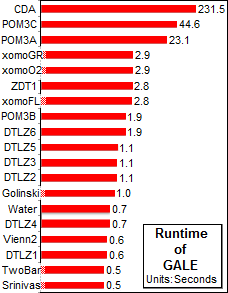
\includegraphics[width=2.25in]{barcharts_runtime_galeAbsolute_v2.png}
\end{center}
\caption{GALE, mean runtime in seconds.}\label{fig:runGale} 
\end{figure}


\begin{figure}[!b]
%\includegraphics[width=2in]{tim/runSpear2.png}\includegraphics[width=1in]{tim/runNsgaii.png}
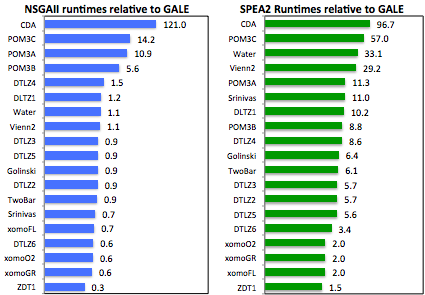
\includegraphics[width=3.45in]{barcharts_runtime_relativeToGale_v2.png}
\caption{NSGA-II, SPEA2, runtimes, relative to GALE (mean values
over all runs) e.g.,
with SPEA2, ZDT1 ran 1.5 times slower than GALE.}\label{fig:runSpea2} 
\end{figure}



\begin{figure}[!b]
%\includegraphics[width=3.5in]{tim/evals.png}
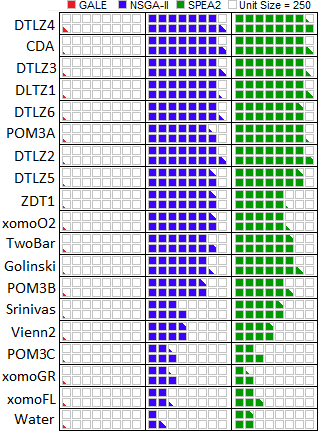
\includegraphics[width=3in]{barcharts_numeval_v2.png}
\caption{Number of evaluations (means over all runs), sorted
by  max. number of evaluations.}\label{fig:evals} 
\end{figure}
%% \begin{figure}[!t]
%% \begin{center}
%% \footnotesize
%% \begin{tabular}{|c@{~}|c@{~}|c@{~}|c@{~}|c@{~}|} \hline
%% Model      & NSGA-II       & GALE       & SPEA2       & Compared  \\ \hline \hline
%% Model      & NSGA-II       & GALE       & SPEA2       &  \\ \hline \hline
%% Golinski   & 1,890         & 32         & 1,270       & 49x     \\ \hline
%% Osyczka2   & 2,850         & 33         & 2,720       & 84x     \\ \hline
%% Schaffer   & 1,650         & 44         & 2,340       & 45x     \\ \hline
%% Srinivas   & 1,850         & 44         & 1,420       & 38x     \\ \hline
%% Tanaka     & 1,740         & 45         & 1,530       & 36x     \\ \hline
%% Viennet2   & 2,500         & 48         & 2,730       & 55x     \\ \hline
%% ZDT1       & 1,300         & 47         & 1,190       & 26x     \\ \hline \hline
%% POM3a      & 3,150         & 43         & 3,470       & 78x     \\ \hline
%% POM3b      & 3,550         & 36         & 3,310       & 95x     \\ \hline
%% POM3c      & 3,040         & 53         & 2,760       & 55x     \\ \hline \hline
%% Median     & 2,195         & 44         & 2,530       & 54x     \\ \hline
%% \end{tabular}
%% \end{center}
%% \caption{Number of Evaluations for each MOEA as averaged across all runs for that model.}
%% \label{fig:numeval}
%% \end{figure}
%% \begin{figure}[!t]
%% \begin{center}
%% \footnotesize
%% \begin{tabular}{|c@{~}|c@{~}|c@{~}|c@{~}|} \hline
%% Model      & NSGA-II     & GALE        & SPEA2 \\ \hline \hline
%% Golinski   & 0.7         & 0.8         & 5.8    \\ \hline
%% Osyczka2   & 0.7         & 0.9         & 5.1    \\ \hline
%% Schaffer   & 0.4         & 0.3         & 28.9   \\ \hline
%% Srinivas   & 0.3         & 0.5         & 7.0    \\ \hline
%% Tanaka     & 0.5         & 0.7         & 7.2    \\ \hline
%% Viennet2   & 0.6         & 0.5         & 16.9   \\ \hline
%% ZDT1       & 0.9         & 3.0         & 4.1    \\ \hline \hline
%% POM3a      & 84.7        & 9.7         & 78.4   \\ \hline
%% POM3b      & 6.8         & 2.2         & 20.8   \\ \hline
%% POM3c      & 140.5       & 14.3        & 107.2  \\ \hline \hline
%% Average    & 23.6        & 3.3         & 28.1   \\ \hline 
%% Median     & 0.7         & 0.9         & 12.1   \\ \hline
%% IQR        & 4.7         & 2.3         & 20.8   \\ \hline
%% \end{tabular}
%% \end{center}
%% \caption{CPU RunTime in seconds for each MOEA as averaged across all runs for that model.}
%% \label{fig:runtime}
%% \end{figure}
 

\subsection{Exploring RQ1 (Speed)}

\fig{runGale} shows GALE's runtimes.
Recall that our models form two groups:
the {\em larger models} include XOMO,POM, CDA
and the {\em smaller maths models} include  ZDT, Golinski, Water, Viennet2,Two-Bar Truss, Srivinas.
As seen in that figure,
most of the smaller models took two seconds, or less,  to optimize.
On the other hand, the larger models took longer (e.g. CDA needed four minutes).









\fig{runSpea2} compares GALE's runtimes to those
of NSGA-II and SPEA2. In that figure, anything with a relative
runtime over 1.0 ran {\em slower} than GALE. Note that 
GALE was faster than SPEA2 for all models. 

For NSGA-II, GALE was a little slower for the smaller models.
However, when for more complex reasoning, GALE ran much faster. 
For the POM3 models, GALE ran up to an order of magnitude faster than both NSGA-II and SPEA2.
As to CDA, GALE ran two orders of magnitude faster (4 minutes versus 7 hours).



\fig{evals}  shows why GALE  runs so much faster than NSGA-II and SPEA2:
NSGA-II and SPEA2 needed between 1,000 and 4,000 evaluations for each model while GALE terminated after roughly 30 to 50 evaluations.
Across every model, SPEA2 and NSGA-II needed between 25 to 100 times more
evaluations to optimize (mean value: 55 times more evaluations).



\subsection{Exploring RQ2 (Quality)}


\subsubsection{CDA}

The above results show GALE running faster than other MOEAs.
While this seems a useful result, it would be irrelevant if
the quality of the solutions found by GALE were much worse than other MOEAs.


One issue with exploring solution quality
with the very slow models like the CDA model was that NSGA-II and SPEA2 ran so slow that 20 runs would 
require nearly an entire week of CPU.
Hence, in this study NSGA-II and SPEA2 were
only run once on CDA.  \fig{cda} shows quality results for the CDA objectives.
Note that GALE achieved the same (or better) minimizations, after far fewer evalautions, than NSGA-II or SPEA2. 


\begin{figure}
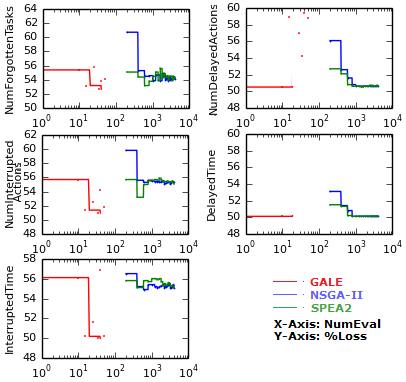
\includegraphics[width=3.3in]{figures/cda.png}
\caption{Execution traces of CDA. X-axis shows number
of evaluations (on a logarithmic scale). 
Solid, colored lines  show  best reductions seen
at each $x$ point.
The y-axis values show percentages of initial values
(so $y=50$ would mean {\em halving} the original value).
For all these
objectives, {\em lower} y-axis values are {\em better}.
}\label{fig:cda} 
\end{figure}


\begin{changed}
\subsubsection{BNH, Golinski, POM3, 
Srinivas, 
Two-Bar Truss, Viennet2, XOMO, and ZDT}

Our other models   were (much)
faster to run.  Hence, for  the other models, we
can offer a more detailed analysis of the quality of
their solutions including hypervolumes and spreads
seen in 20 repeated runs.
\begin{figure}
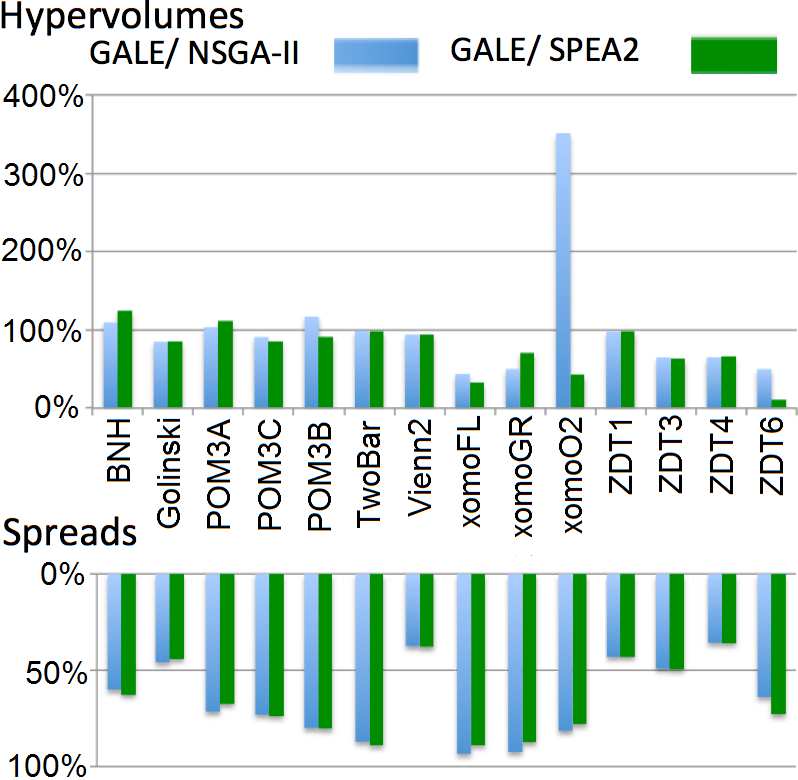
\includegraphics[width=3.15in]{mathsModelsResults.png}
\caption{Quality results from BNH, Golinski, POM3, Two-Bar Truss, Viennet2, XOMO, ZDT.
All numbers are ratios of mean hypervolumes and spreads achieved in 20 repeated runs of GALE, NSGA-II and SPEA2.
At 100\%, the mean hypervolumes and spreads achieved by GALE are the same as the other optimizers.
In this figure,  {\em better} hypervolumes are {\em larger} while {\em better} spreads are {\em smaller}.}\label{fig:rmodels}
\end{figure}
\begin{figure}[!t]
\scriptsize
\centering
\begin{tabular}{|r|c|c|c|c|} \hline
	&	Model	&	NSGA-II	&	GALE	&	SPEA2	\\ \hline
%DTLZ	&	DTLZ1-d5-o2	&	62\%	&	70\%	&	\colorbox{lightgray}{61\%}	\\
%Toolkit	&	DTLZ1-d5-o4	&	\colorbox{lightgray}{78\%}	&	83\%	&	\colorbox{lightgray}{78\%}	\\
%	&	DTLZ2-d10-o2	&	65\%	&	73\%	&	\colorbox{lightgray}{64\%}	\\
%	&	DTLZ2-d10-o4	&	86\%	&	86\%	&	\colorbox{lightgray}{80\%}	\\
%	&	DTLZ3-d10-o2	&	65\%	&	73\%	&	\colorbox{lightgray}{64\%}	\\
%	&	DTLZ3-d10-o4	&	81\%	&	85\%	&	\colorbox{lightgray}{79\%}	\\
%	&	DTLZ4-d10-o2	&	70\%	&	90\%	&	\colorbox{lightgray}{67\%}	\\
%	&	DTLZ4-d10-o4	&	93\%	&	92\%	&	\colorbox{lightgray}{90\%}	\\
%	&	DTLZ5-d10-o2	&	66\%	&	76\%	&	\colorbox{lightgray}{64\%}	\\
%	&	DTLZ5-d10-o4	&	80\%	&	84\%	&	\colorbox{lightgray}{79\%}	\\
%	&	DTLZ6-d20-o2	&	67\%	&	71\%	&	\colorbox{lightgray}{67\%}	\\
%	&	DTLZ6-d20-o4	&	83\%	&	85\%	&	\colorbox{lightgray}{81\%}	\\ \hline
xomo 	&	xomofl-d27-o4	&	96\%	&	\colorbox{lightgray}{89\%}	&	96\%	\\
models	&	xomogr-d27-o4	&	97\%	&	\colorbox{lightgray}{89\%}	&	97\%	\\
%	&	xomoos-d27-o4	&	97\%	&	\colorbox{lightgray}{88\%}	&	97\%	\\
	&	xomoo2-d27-o4	&	96\%	&	\colorbox{lightgray}{89\%}	&	97\%	\\
%	&	xomoal-d27-o4	&	96\%	&	\colorbox{lightgray}{87\%}	&	96\%	\\ \hline
POM3 	&	POM3A-d9-o4	&	92\%	&	91\%	&	\colorbox{lightgray}{89\%}	\\
models	&	POM3B-d9-o4	&	92\%	&	\colorbox{lightgray}{90\%}	&	\colorbox{lightgray}{89\%}	\\
	&	POM3C-d9-o4	&	96\%	&	\colorbox{lightgray}{94\%}	&	96\%	\\ \hline
Constrained	&	BNH-d2-o2	&	98\%	&	\colorbox{lightgray}{75\%}	&	97\%	\\
%&	Osyczka2-d6-o2	&	77\%	&	\colorbox{lightgray}{69\%}	&	78\%	\\
maths&	Srinivas-d2-o2	&	95\%	&	\colorbox{lightgray}{80\%}	&	95\%	\\
%	&	Tanaka-d2-o2	&	\colorbox{lightgray}{84\%}	&	85\%	&	85\%	\\
models	&	TwoBarTruss-d3-o2	&	95\%	&	\colorbox{lightgray}{78\%}	&	95\%	\\
	&	Water-d3-o5	&	95\%	&	\colorbox{lightgray}{90\%}	&	95\%	\\ \hline
Unconstrained	&	Golinski-d7-o2	&	81\%	&	\colorbox{lightgray}{65\%}	&	81\%	\\
math	&	Viennet2-d2-o3	&	\colorbox{lightgray}{73\%}	&	\colorbox{lightgray}{73\%}	&	\colorbox{lightgray}{73\%}	\\
%&	Viennet3-d2-o3	&	88\%	&	\colorbox{lightgray}{78\%}	&	88\%	\\
%	&	Viennet4-d2-o3	&	90\%	&	\colorbox{lightgray}{77\%}	&	89\%	\\
models	&	ZDT1-d30-o2	&	85\%	&	\colorbox{lightgray}{81\%}	&	85\%	\\
	&	ZDT2-d30-o2	&	\colorbox{lightgray}{73\%}	&	\colorbox{lightgray}{72\%}	&	\colorbox{lightgray}{73\%}	\\
	&	ZDT3-d30-o2	&	84\%	&	\colorbox{lightgray}{80\%}	&	85\%	\\
	&	ZDT4-d10-o2	&	\colorbox{lightgray}{68\%}	&	74\%	&	\colorbox{lightgray}{69\%}	\\
	&	ZDT6-d10-o2	&	71\%	&	72\%	&	\colorbox{lightgray}{69\%}	\\ \hline
\end{tabular}
\caption{Median scores comparing final frontier values to
initial populations. Calculated using Equation 1. Lower
scores are better. Gray cells are significantly different
(statistically) and better than the other values in that row.
In the models column, model name shows objectives and decisions;
e.g. d27-o4 means
the model has 27 decisions and 4 objectives.  }
\label{fig:whateveryouwannacallme}
\end{figure}

For example, \fig{rmodels} shows the ratio of mean hypervolumes 
and spreads found in 20 repeated runs of three optimizers. All numbers are ratios of GALE's results divided
by either NSGS-II or SPEA2.  

The Srivinas, POM3c and ZDT2 results were
excluded from \fig{rmodels} after an A12 effect size test
reported a ``small effect'' for the performance deltas between GALE and the other optimizers.
All the other results have the property that $\mathit{A12} \ge 0.6$; i.e. they are not trivially small
differences
  (this A12
  test was recently endorsed by Arcuri and
  Briand at ICSE'11~\cite{arcuri11} as an
  appropriate test to check for trivially small
  differences when studying stochastic processes).

\fig{rmodels} shows that for $\frac{5}{17}$
of the smaller maths models (XOMO FL, XOMO GR, and
ZDT346) GALE's hypervolumes were much lower than the
other optimizers.  On the other hand, GALE's
hypervolumes are comparable, or better, for most of
the small maths models: \bi
\item
GALE does better than NSGA-II in BNH, POM3a, POM3b and XOMO
O2.
\item As seen in 
\fig{rmodels}, the hypervolumes are very similar for Two-Bar Truss,
Viennet2 and ZDT1.  
\item
Also, as mentioned
above the Srivinas and POM3c and ZDT2 results were only trivially different.
\ei
Other quality indicators offer other evidence for
the
value of GALE's reasoning. For example, \fig{rmodels} shows that GALE
consistently achieves lower and better spreads than the other optimizers.

As to the {\em improvement}, 
 \fig{whateveryouwannacallme} shows the
Equation~1 {\em loss} values between members of the
first and final population generated by different
optimizers. In that figure,
 gray cells are significantly different
(statistically) and better (less is better in that figure)
than the other values in that row
(for statistics, we used Mann-Whitney, 95\%
confidence to test significance, then used A12 to
mark as non-gray any differences that were just
small effects). Note that, in the majority case, GALE's results
are amongst the best for all the optimizers used in this study.


\end{changed}



\begin{changed}

\begin{figure}
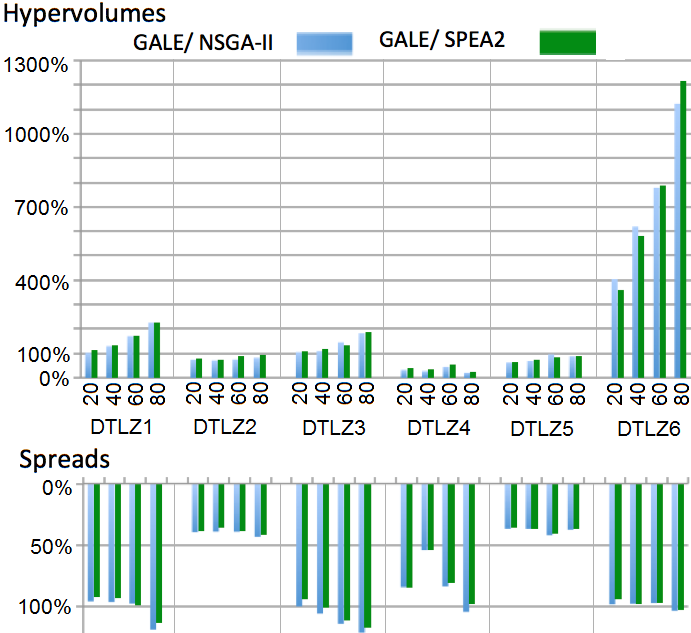
\includegraphics[width=3.25in]{dtlzResults1.png}
\caption{Quality results from DTLZ with 20 decisions and two objectives.
Same format as \fig{rmodels}; i.e. better hypervolumes are {\em larger} while {\em better} spreads are {\em smaller}.}\label{fig:dtlz}
\end{figure}
\begin{figure*}[!b]
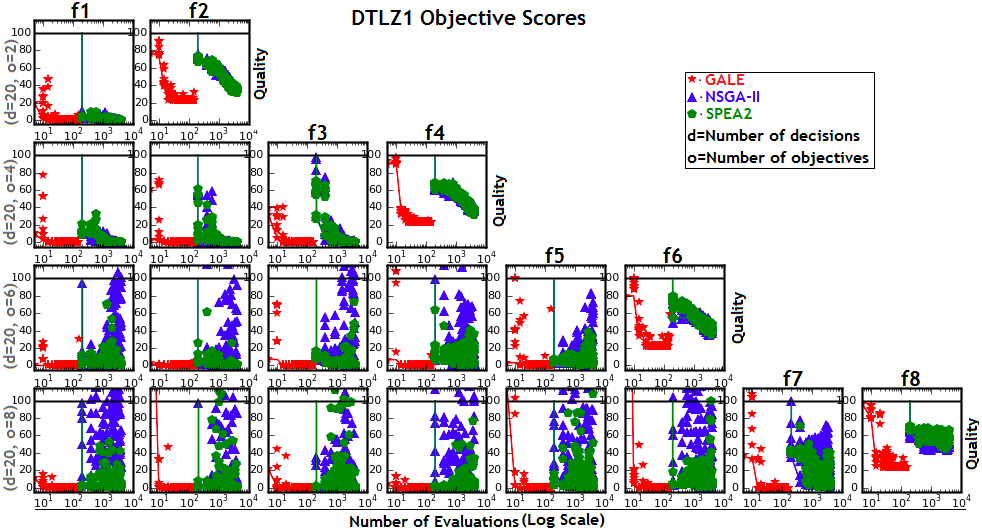
\includegraphics[width=6.8in]{dtlzResults2.png}
\caption{DTLZ1; d=20, o=2,4,6,8.
Each column is one objective f1,f2,...f8. Colors indicate results
for different optimizers:
GALE results are in 
\textcolor{red}{{\bf RED}},
NSGA-II results are in 
 \textcolor{blue}{{\bf BLUE}},
and the SPEA2 results are shown in 
  \textcolor{darkgreen}{{\bf GREEN}}
(and the 
red,blue, or green lines show the best solution found so far for each
objective for GALE, NSGA-II, and SPEA2 respectively). 
The x-axis of these
plots shows the number of evaluations seen during optimization.
All objective scores are expressed as percentages
of the mean objective scores seen in the baseline population before any optimization
(this baseline is shown as 100\% on the y-axis of all these plots). 
For these objectives, {\em better} scores are {\em smaller}.
}\label{fig:o2468}
\end{figure*}



\subsubsection{DTLZ}

 DTLZ  can be configured to include varying number of decisions
and objectives.  
Our first DTLZ study used two objectives and  {\em changed the number of decisions} from 20 to 80. The other study used twenty decisions and  {\em changed
the number of objectives} from two to eight. We found
 runtime issues with  computing hypervolume for models with many objectives
 so  the  second study  explored one DTLZ model selected at random (DTLZ1).

The results of both studies are shown in \fig{dtlz}
and \fig{o2468}. Note that the differences
between all treatments were not considered ``small'' effects (via A12).

\fig{dtlz} shows results from changing the number of decisions.
GALE's spreads are never much worse than the other
optimizers, and often they are much
better. 
As to the hypervolumes in  \fig{dtlz}:
\bi
\item
A rising ``staircase'' was observed as the number of
objectives was increased. That is,  GALE did {\em better}
as the problem grew more complex (i.e. the number the decisions increased).
\item
Sometimes, GALE does much better on hypervolumes as
seen in the DTLZ6 results.
\ei
\fig{o2468} shows results from increasing the
number of objectives. 
In those results,   GALE 
finds minimal values for all objectives and does
so using  orders of magnitude fewer evaluations than
 other optimizers.
 \addit{xomoresults}




\subsubsection{Summary of Results from Maths Models}

These results from our smaller maths models all show similar trends.
GALE's truncated search sometimes explores a
smaller set of solutions than other
optimizers.  Hence, as one might have expected, GALE's hypervolumes can be smaller than other optimizers. On the other hand,
within the volume it does explore, GALE seems to spread
out more that other optimizers.
Since GALE takes more care to explore its volume of solutions,
it can find better solutions (with most improvement to the objective scores)
than other optimizers.
\end{changed}

%\begin{figure}
%{\s%% mall
%% \begin{tabular}{r@{~}|r@{~}|r@{~}|r@{~}|r@{~}|r@{~}|r}
%%              & \multicolumn{2}{c}{Hypervolumes}       & \multicolumn{2}{c}{Spreads}           & 
%% \multicolumn{2}{c}{Evaluations}\\	
%%          o    & $\frac{\mathit{gale}}{\mathit{spea2}}$  & $\frac{\mathit{gale}}{\mathit{NSGA-II}}$ & $\frac{\mathit{gale}}{\mathit{spea2}}$ & $\frac{\mathit{gale}}{\mathit{NSGA-II}}$ & 
%% $\frac{\mathit{gale}}{\mathit{spea2}}$ & $\frac{\mathit{gale}}{\mathit{NSGA-II}}$\\\hline
%% 2 & 106       & 111      & 100      & 100      & 4187     & 4202\\
%% 4 & 99        & 106      & 93       & 109      & 3886     & 4072\\
%% 6 & 104       & 106      & 139      & 145      & 3268     & 1712\\
%% 8 & 153       & n/a        & 180      & n/a        & 182      & n.a
%% \end{tabular}
%% }
%% \caption{More quality results from DTLZ with 20 decisions and 





%dtlz d-X0-o2 experiment

%{\scriptsize
%\begin{tabular}{r|r|r|r}
%            algorithm         &  nsga-II&	spea2 &	gale\\\hline
%number of evaluations &  48,260 &	 49,710 &	 928 \\
%evaluations, as a ration of GALE & 53 &	55 & 1
%\end{tabular}}
%% \begin{figure}
%% \begin{center}
%% \footnotesize
%% \begin{tabular}{lc@{~}|c@{~}|c@{~}|c@{~}} 
%% Type&Model      & NSGA-II      & GALE         & SPEA2 \\ \hline 
%% small&Golinski   & 76\%         & \colorbox{lightgray}{68\%}         & 74\%  \\ 
%% &Osyczka2   & 75\%         & \colorbox{lightgray}{72\%}         & 75\%  \\ 
%% &Schaffer   & \colorbox{lightgray}{62\%}         & 63\%         & \colorbox{lightgray}{62\%}  \\ 
%% &Srinivas   & 94\%         & \colorbox{lightgray}{84\%}         & 94\%  \\ 
%% &Tanaka     & 84\%         & \colorbox{lightgray}{75\%}         & 84\%  \\ 
%% &Viennet2   & \colorbox{lightgray}{73\%}         & 75\%         & \colorbox{lightgray}{73\%}  \\
%% &ZDT1       & 87\%         & \colorbox{lightgray}{80\%}         & \colorbox{lightgray}{82\%}  \\ \hline 
%% medium &POM3a      & 92\%         & 91\%         & \colorbox{lightgray}{90\%}  \\
%% &POM3b      & 91\%         & \colorbox{lightgray}{90\%}         & \colorbox{lightgray}{90\%}  \\ 
%% &POM3c      & 93\%         & 90\%         & 93\% 
%% \end{tabular}
%% \end{center}
%% \caption{Median scores comparing final frontier values
%% to initial populations. Calculated using \eq{cdom}.
%% {\em Lower} scores are {\em better}.
%% Gray cells are significantly
%% different (statistically) and better than the other values in that row.}
%% \label{fig:scores}
%% \end{figure}








\begin{figure*}[!t]
 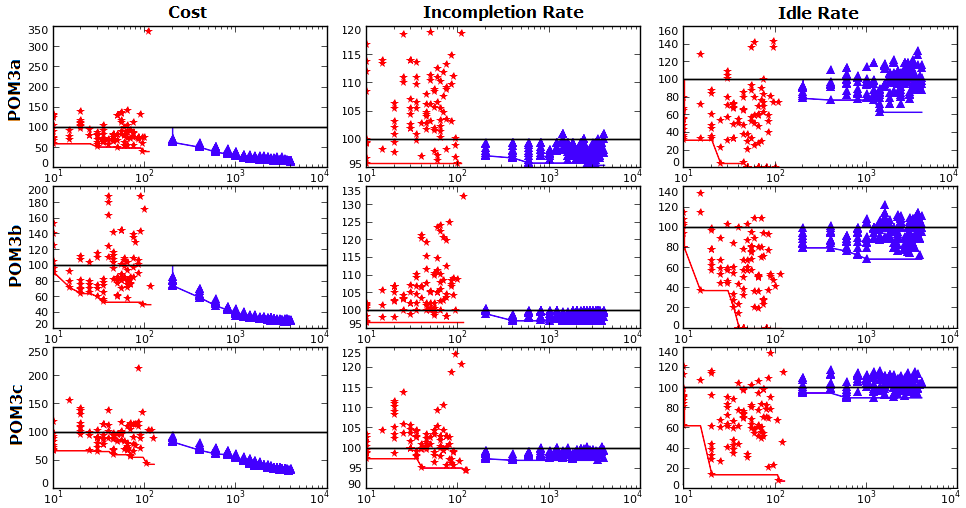
\includegraphics[width=7in]{figures/figure_analytics_obj_score_plots.png}
\caption{POM results: 20 repeats of each MOEA (one row
per scenario). Same format as \fig{xomoresults}' i.e.
GALE results are in 
\textcolor{red}{{\bf red}}
and NSGA-II results are in 
 \textcolor{blue}{{\bf blue}}. Each x-axis shows number of evaluations (log scale).
On the y-axis, results are expressed
as percentages of the median value seen in the  initial baseline population. 
For all objectives, lower is better and the solid line shows
the best results seen so far on any objective.    }
\label{fig:zdt1objspace}
\end{figure*}


\subsection{POM3 and XOMO}

\fig{whateveryouwannacallme} showed a statistical comparison of the improvements
achieved between the first and final generations
of GALE, NSGA-II and SPEA2 for the POM3 and XOMO models.
Apart from the statistical analysis, it is also insightful
to look at the changes in the raw objective scores.

\fig{xomoresults} and 
\fig{zdt1objspace} show  how NSGA-II and GALE evolved candidates
with better objective scores for the XOMO and POM3 models.
The format of these figures is the same as \fig{o2468}.
That is,
the y-vertical-axis denotes
changes from the median of the initial population.
Hence, $Y=50$ would indicate that we have halved the value of some objective;
while  $Y \gt 100$ would indicate that optimization failed to improve this objective.

In both \fig{xomoresults} and \fig{zdt1objspace}, all 
the y-axis values are computed such that {\em lower}
values are {\em better}. For example, the results in the column
labeled {\em Incompletion Rate} of \fig{zdt1objspace}
is the ratio {\em initial/now} values. Hence, if we are {\em now} completing a larger
percentage of the requirements, then {\em incompletion} is better if it is
less than 100\%; i.e. \[\mathit{Incompletion}\% = 100 - \mathit{Completion}\%\]


\begin{changed}
\noindent 
In terms of advocating for GALE,
the \fig{xomoresults} results for the XOMO model
are unequivocal: on all dimensions, for all runs of the model,
GALE finds decisions that leads to lower  (i.e.  better) objective scores than NSGA-II.
Further, as shown on the x-axis, GALE does so using far fewer evaluations than NSGA-II.
\end{changed}

As to the \fig{zdt1objspace} results from POM3, these results are---at first glance---somewhat surprising.
These results seem to say  say that GALE
performed worse than NSGA-II since NSGA-II achieved larger
{\em Cost} reductions. However, the {\em Idle}
results  show otherwise:
 NSGA-II rarely reduced
the {\em Idle} time of the developers  while GALE
found ways to achieve reductions down to near zero percent {\em Idle}.

This observation begs the question: in \fig{zdt1objspace},
how could NSGA-II reduce cost while keeping developers working at the same rate
(i.e. not decrease developer {\em
  Idle} time)?  We checked the model outputs
and realized that  NSGA-II's advice to developers was to
complete
fewer requirements. This is an interesting quirk of pricing models in the agile
community- if developers are rewarded for quickly completing tasks, they will
favor the easier ones, leaving the slower and harder tasks to other developers (who
will get rewarded less). 
Note that this is not necessarily an error in the  POM3 costing routines- providing 
that an optimizer also avoids leaving programmers idle.
In this regard, NSGA-II is far worse than GALE since the latter
successfully reduces {\em cost} as well as the {\em Idle Rate}.




\subsection{Answers to Research Questions}

{\bf RQ1 (speed):} {\em Does GALE terminate faster than other MOEA tools?}:

Note that 
for  smaller models, GALE was slightly slower than NSGA-II (but much faster than 
SPEA2). Also, for large models like CDA, GALE was much faster.
These two effects result from the relative complexity
of (a)~model evaluation versus (b)~GALE's internal clustering of the data.
When model evaluation is very fast, the extra time needed for clustering
dominates the runtimes of GALE.  However, when the
model evaluation is very long, the time
needed for GALE's clustering is dwarfed by the evaluation costs. Hence,
GALE is strongly recommended for models that require long execution times.
Also, even though GALE is slower for smaller models, we would still recommend GALE 
for those small models.
The delta between absolute runtimes of GALE and the other optimizers is negligible 
($\le 3$ seconds).
Further, GALE requires fewer evaluations thus reducing the complexity
for anyone working to understand the reasoning (e.g.  a
programmer conducting system tests on a new model).

{\bf RQ2 (quality):} {\em Does  GALE  return  similar or better solutions than other MOEA tools?}:

GALE's solutions are rarely worse than other optimizers, and sometimes, they are 
better (and note that the generality of this claim is explored futher in \tion{ob}.).


\section{Threats to Validity}


\subsection{Optimizer Bias}\label{sec:ob}
While we have shown that GALE does better than NSGA-II and SPEA2, we have not shown
that it works better than {\em all} optimizers. Hence, one source of bias in this
study is the selection of comparison algorithms.

As mentioned in our Frequently Asked Questions list of~\tion{faq}, 
it is theoretically impossible to show that any optimizer is better than all others.
All that is achievable in one study is a limited comparison between select optimizers. 
In this work, GALE was compared to 
NSGA-II and SPEA2. Our reasons for
selecting these two were discussed in
\tion{compares}.  Future work should compare GALE to other optimizers.

\subsection{ Sampling Bias}
This bias threatens any conclusion based on the
analysis of a finite number of optimization
problems.  Hence, even though GALE runs well on
the models studied here, there may well be other
models that could defeat GALE.  

For this issue of sampling bias, the best we can do
is define our methods and publicize our tools so
that other researchers can try to repeat our results
and, perhaps, point out a previously unknown bias in
our analysis. Hence, all the experiments (except for
CDA) in this paper are made available online (see \tion{avail}).  Hopefully, other
researchers will emulate our methods to repeat,
refute, or improve our results.


\subsection{Parameter Bias}
For this study, we did not do extensive parameter tuning:
NSGA-II and SPEA2 were run using their default settings
while GALE was run using the settings that worked well on the first model we
studied, which were then frozen for the
rest of this study. As documented above, those parameters were:
\bi
\item $\mu$ = 100:  population size;
\item $\omega$ = $\sqrt{\mu}$: minimum size leaf clusters;
\item $\lambda = 3$: premature stopping criteria (sets the
maximum allowed 
generations without
any improvement on any objective).
\item   $\Delta=1$: the ``accelarator'' that encourages larger mutations;
\item  $\gamma=1.5$: the ``brake'' that blocks excessive mutation.
\ei
(Note that these were constant across all our studies except for the DTLZ models which used
$\Delta=4$).

If this paper was arguing that these parameters were somehow {\em optimal},
then it would be required to present experiments defending the above settings.
However, our  claim is less than that- we only aim  to show
that with these settings, GALE does as well than standard
MOEA tools. In future work, we will explore other  settings.



   
\section{Conclusions}
This paper has introduced GALE, an evolutionary
algorithm that combines active learning with
continuous domination functions and fast spectral
learning to find a response surface model; i.e. a
set of approximations to the Pareto frontier.


We showed that for a range of scenarios and models
that GALE found solutions equivalent or better than
standard methods (NSGA-II and SPEA2).  Also, those
solutions were found using one to two orders of
magnitude fewer evaluations.

\begin{changed}
As mentioned above, one repeated result was
that
GALE's truncated search sometimes explores a
smaller set of solutions than other
optimizers: hence, it can sometimes generate lower hypervolumes.
However, for the space it does explore,
GALE seems to do a better job than other optimizers.
A repeated result in the above is that GALE's solutions are more spread out
than other optimizers so 
 it 
can find better solutions (with most improvement to the objective scores).
\end{changed}

We claim that GALE's superior performance is due to
its better understanding of the shape of the Pareto
frontier.  Standard MOEA tools generate too many
solutions since they explore uninformative parts of
the solution space.  GALE, on the other hand, can
faster find best solutions across that space since
it understands and exploits the shape of the Pareto
frontier.


These results suggest that it is perhaps time to reconsider the random
mutation policy used by most MOEAs.  GALE can navigate the space of
options using far fewer evaluations than the random mutations of
NSGA-II and SPEA2. We would propose a ``look before you leap'' policy;
i.e. before applying some MOEA like SPEA2 or NSGA-II, cluster the
known solutions and look for mutation directions in the non-dominated
clusters.

   


\section*{Acknowledgements}
\begin{changed}
The authors wish to thank the anonymous reviewers of this
paper for their many excellent suggestions on how to improve this paper.
\end{changed}
The work was funded by NSF grant CCF:1017330 and the
Qatar/West Virginia University research grant NPRP
09-12-5-2-470.  This research was partially
conducted at NASA Ames Research Center. 

Reference
herein to any specific commercial product, process,
or service by trade name, trademark, manufacturer,
or otherwise, does not constitute or imply its endorsement by the United States Government.


    
    %\underline{{\bf FINAL SCORING:}}
    %The POM models score a planning policy by comparing a developers' {\em %incremental} decisions
    %to those that might have been made by some omniscient developer (that has access
    %to the   {\em final} cost and priority of requirements).

\color{MyDarkBlue}
\section*{Appendix}
The maths models used in this paper are shown in the next few pages.
\color{black}

\begin{figure*}[!t]\scriptsize
\color{MyDarkBlue}
        \centering
                \begin{tabular}{ | l | c | l@{~} | c@{~} | }
                \hline
                \multicolumn{4}{ | c@{~} | }{Unconstrained Multi-Objective Functions}\\
                \hline
                Name & n & Objectives & Variable Bounds\\\hline\hline
                
                
                
                Golinksi & 7 & \begin{tabular}{ l@{~} }
                {$ r = 0.7854$} \\
                {$ s = 14.933$} \\
                {$ t = 43.0934$} \\
                {$ u = -1.508$} \\
                {$ v = 7.477$} \\
                {$ A(\vec{x}) = r x_1 x_2^2 (\frac{10 x_3^2}{3.0} + s x_3 - t) $}\\
                {$ B(\vec{x}) = u x_1 (x_6^2 + x_7^2)+ v(x_6^3 + x_7^3) + r(x_4*x_6^2 + x_5*x_7^2) $}\\
                {$ aux(\vec{x}) = 745.0 \frac{x_4}{x_2 * x_3} $}\\
                {$ f_1(\vec{x})= A + B $}\\
                {$ f_2(\vec{x})= \frac{\sqrt{aux^2 + 1.69e7}}{0.1 x_6^3} $}
                \end{tabular} & \begin{tabular}{ c@{~} }
                {$ 2.6 <= x_1 <= 3.6 $}\\
                {$ 0.7 <= x_2 <= 0.8 $}\\
                {$ 17.0 <= x_3 <= 28.0 $}\\
                {$ 7.3 <= x_4, x_5 <= 8.3 $}\\
                {$ 2.9 <= x_6 <= 3.9 $}\\
                {$ 5.0 <= x_7 <= 5.5 $} \\
                \end{tabular} \\
                \hline

                Viennet 2 & 2 & \begin{tabular}{ l@{~} }
                {$ f_1(\vec{x})= \frac{(x_1-2)(x_1-2)}{2} + \frac{(x_1+1)(x_1+1)}{13} + 3 $}\\
                {$ f_2(\vec{x})= \frac{(x_1+x_2-3)(x_1+x_2-3)}{36} + \frac{(-x_1+x_2+2)(-x_1+x_2+2)}{8} - 17 $}\\
                {$ f_3(\vec{x})= \frac{(x_1+2x_2-1)(x_1+2x_2-1)}{175} + $} \\ 
                {$ \frac{(2x_2-x_1)(2x_2-x_1)}{17} - 13 $} \\
                \end{tabular} & {$ -4 <= x_i <= 4 $}\\
                \hline
                
                %% Viennet 3 & 2 & \begin{tabular}{ l@{~} }
                %% {$ A(\vec{x}) = 3*x_1 - 2*x_2 + 4        $}\\
                %% {$ B(\vec{x}) = x_1 - x_2 + 1              $}\\
                %% {$ f_1(\vec{x})=  0.5 * (x_1^2 + x_2^2) + sin(x_1^2 + x_2^2)   $}\\
                %% {$ f_2(\vec{x})= \frac{A^2  }{ 8 + \frac{B^2}{27} + 15 }      $}\\
                %% {$ f_3(\vec{x})= \frac{1}{x_1^2 + x_2^2+1} - 1.1 * e^{-(x_1^2) - (x_2^2)}    $} 
                %% \end{tabular} & {$ -3 <= x_i <= 3 $}\\
                %% \hline

                %% Viennet 4 & 2 & \begin{tabular}{ l@{~} }
                %% {$ f_1(\vec{x})= \frac{(x_1-2)(x_1-2)}{2} + \frac{(x_1+1)(x_1+1)}{13} + 3 $}\\
                %% {$ f_2(\vec{x})= \frac{(x_1+x_2-3)(x_1+x_2-3)}{175} + \frac{(2*x_2-x_1)*(2*x_2-x_1)}{17} - 13 $}\\
                %% {$ f_3(\vec{x})= \frac{(3*x_1-2*x_2+4) * ( 3*x_1-2*x_2+4)}{8}   +      $} \\ 
                %% {$ \frac{(x_1-x_2+1)(x_1-x_2+1)}{27} + 15 $} \\
                %% \end{tabular} & {$ -4 <= x_i <= 4 $}\\
                %% \hline

                ZDT1 & 30 & \begin{tabular}{ l@{~} }
                {$ f_1(\vec{x})= x_1 $}\\
                {$ f_2(\vec{x})=  g * (1 - \sqrt{\frac{x_1}{g}})$}\\
                {$ g(\vec{x}) = 1 + \frac{9}{n-1}\sum_{i=2}^{n}(x_i) $}
                \end{tabular} & {$ 0 <= x_i <= 1 $}\\
                \hline

                ZDT2 & 30 & \begin{tabular}{ l@{~} }
                {$ f_1(\vec{x})= x_1 $}\\
                {$ f_2(\vec{x})=  g * (1 - (\frac{x_1}{g})^2)$}\\
                {$ g(\vec{x}) = 1 + \frac{9}{n-1}\sum_{i=2}^{n}(x_i) $}
                \end{tabular} & {$ 0 <= x_i <= 1 $}\\
                \hline
                
                ZDT3 & 30 & \begin{tabular}{ l@{~} }
                {$ f_1(\vec{x})= x_1 $}\\
                {$ f_2(\vec{x})=  g * (1 - \sqrt{(\frac{x_1}{g})} - \frac{x_1}{g} * sin(10*\pi*x_1) )$}\\
                {$ g(\vec{x}) = 1 + \frac{9}{n-1}\sum_{i=2}^{n}(x_i) $}
                \end{tabular} & {$ 0 <= x_i <= 1 $}\\
                \hline
                
                ZDT4 & 10 & \begin{tabular}{ l@{~} }
                {$ f_1(\vec{x})= x_1 $}\\
                {$ f_2(\vec{x})=  g * (1 - \sqrt{(\frac{x_1}{g})} - \frac{x_1}{g} * sin(10*\pi*x_1) )$}\\
                {$ g(\vec{x}) = 1 + 10*(n-1) + \sum_{2}^{n} (x_i^2 - 10*cos(4*\pi*x_i)) $} \\
                \end{tabular} & \begin{tabular}{ c@{~} }
                {$ 0 <= x_1 <= 1 $}\\
                {$ -5 <= x_2,...,x_{10} <= 5$}\\
                \end{tabular}\\
                \hline
                
                ZDT6 & 10 & \begin{tabular}{ l@{~} }
                {$ f_1(\vec{x})=  1 - e^{-4*x_1} * sin(6*\pi*x_1)^6         $}\\
                {$ f_2(\vec{x})=  g * (1  - (\frac{f_1(\vec{x})}{g})^2)  $} \\
                {$ g(\vec{x}) = 1 + 9 * \frac{  \sum_{2}^{n} x_i    }{(n-1)^{0.25}}     $} \\
                \end{tabular} & {$ 0 <= x_i <= 1 $}\\
                \hline


                \end{tabular}
                \caption[Defining the Unconstrained Math Models]{Unconstrained standard maths
models. All objectives
are to be minimized unless otherwise denoted.}
        \label{fig:uncon}

\end{figure*}


\begin{figure*}
\scriptsize
\color{MyDarkBlue}
        \centering
                \begin{tabular}{ | l | c | l@{~} | l@{~} | c@{~} | }
                        \hline
                        \multicolumn{5}{ | c@{~} | }{Constrained Multi-Objective Functions}\\
                        \hline
                        Name & n & Objectives & Constraints & Variable Bounds\\\hline \hline    
                        
                        BNH & 2 & \begin{tabular}{ l@{~} }
                                {$ f_1(\vec{x}) = 4*x_1^2 + 4x_2^2 $}\\
                                {$ f_2(\vec{x}) = (x_1-5)^2 + (x_2-5)^2 $}\end{tabular} & \begin{tabular}{ l@{~} }
                                {$ g_1(\vec{x}) = ( (x_1-5)^2 + 2*x_2^2) <= 25 $}\\
                                {$ g_2(\vec{x}) = ( (x_1-8)^8 + (x_2 + 3)^2 ) >=7.7 $}\end{tabular} & \begin{tabular}{ c@{~} }
                                {$ 0 <= x_1 <= 5 $}\\
                                {$ 0 <= x_2 <= 3$}\\
                                \end{tabular}\\ \hline
                                
                        %% Osyczka 2 & 6 & \begin{tabular}{ l@{~} }
                        %%         {$ A(\vec{x}) = 25 (x_1 - 2)^2 + (x_2 - 2)^2 $}\\
                        %%         {$ B(\vec{x}) =  (x_3 - 1)^2*(x_4 - 4)^2 +$}\\
                        %%         {$ (x_5 - 2)^2$}\\
                        %%         {$ f_1(\vec{x}) =  0 - A - B  $}\\
                        %%         {$ f_2(\vec{x}) = x_1^2 + x_2^2 + x_3^2 + $}\\
                        %%         {$ x_4^2 + x_5^2 + x_6^2 $} \end{tabular} & \begin{tabular}{ l@{~} }
                        %%         {$ g_1(\vec{x}) = x_1 + x_2 - 2 >= 0 $}\\
                        %%         {$ g_2(\vec{x}) = 6 - x_1 - x_2 >= 0 $}\\
                        %%         {$ g_3(\vec{x}) = 2 - x_2 + x_1 >= 0 $}\\
                        %%         {$ g_4(\vec{x}) = 2 - x_1 + 3 x_2 >= 0 $}\\
                        %%         {$ g_5(\vec{x}) = 4 - (x_3-3)^2 - x_4 >= 0 $}\\
                        %%         {$ g_6(\vec{x}) = (x_5-3)^3 + x_6 - 4 >= 0$}\end{tabular} & \begin{tabular}{ c@{~} }
                        %%                 {$ 0 <= x_1,x_2,x_6 <= 10 $}\\
                        %%                 {$ 1 <= x_3,x_4 <= 5 $}\\
                        %%                 {$ 0 <= x_5 <= 6 $}
                        %%         \end{tabular}\\ \hline
                                
                        Srinivas & 2 & \begin{tabular}{ l@{~} }
                                {$ f_1(\vec{x}) = (x_1 - 2)^2 + (x_2-1)^2 + 2 $}\\
                                {$ f_2(\vec{x}) = 9x_1 - (x_2 -1)^2 $}\end{tabular} & \begin{tabular}{ l@{~} }
                                {$ g_1(\vec{x}) = x_2 + 9x_1 >= 6 $}\\
                                {$ g_2(\vec{x}) = -x_2 + 9x_1 >= 1 $}\end{tabular} & {$ -20 <= x <= 20 $}\\\hline

                        %% Tanaka & 2 & \begin{tabular}{ l@{~} }
                        %%         {$ f_1(\vec{x}) = x_1 $}\\
                        %%         {$ f_2(\vec{x}) = x_2 $}\end{tabular} & \begin{tabular}{ l@{~} }
                        %%         {$ A(\vec{x}) = 0.1 \cos{(16\arctan{(\frac{x_1}{x_2})})} $}\\
                        %%         {$ g_1(\vec{x}) = 1 - x_1^2 - x_2^2 + A <= 0 $}\\
                        %%         {$ g_2(\vec{x}) = (x_1 - 0.5)^2 + $}\\
                        %%         {$ (x_2 - 0.5)^2 <= 0.5 $}\end{tabular} & {$ -\pi <= x <= \pi $}\\\hline
                                
                        Two-bar Truss & 3 & \begin{tabular}{ l@{~} }
                                {$ s_1(\vec{x}) = \frac{20*\sqrt{16+x_3^2}}{(x_1*x_3)}    $} \\
                                {$ s_2(\vec{x}) = \frac{80*\sqrt{1+x_3^2}}{(x_2*x_3)}    $} \\
                                {$ f_1(\vec{x}) = x_1 * \sqrt{16*x_3^2} + x_2*\sqrt{1+x_3^2} $}\\
                                {$ f_2(\vec{x}) = max(s_1, s_2) $}\end{tabular} & \begin{tabular}{ l@{~} }
                                {$ s_1(\vec{x}) = \frac{20*\sqrt{16+x_3^2}}{(x_1*x_3)}    $} \\
                                {$ s_2(\vec{x}) = \frac{80*\sqrt{1+x_3^2}}{(x_2*x_3)}    $} \\
                                {$ g_1(\vec{x}) = ( max(s_1, s_2) ) <= 100000 $} \end{tabular} & \begin{tabular}{ c@{~} }
                                {$ 0 <= x_1,x_2 <= 0.01 $}\\
                                {$ 1 <= x_3 <= 3$}\\
                                \end{tabular}\\ \hline

                        Water & 3 & \begin{tabular}{ l@{~} }
                                {$ f_1(\vec{x}) = 106780.37*(x_2+x_3) + 61704.67$}\\
                                {$ f_2(\vec{x}) = 3000*x_1 $}\\
                                {$ f_3(\vec{x}) = \frac{(305700*2289*x_2)}{((0.06*2289)**0.65)} $}\\
                                {$ E(\vec{x}) = e^{-39.75*x_2+9.9*x_3+2.74} $}\\
                                {$ f_4(\vec{x}) = 250*2289*x_2*E(\vec{x}) $}\\
                                {$ f_5(\vec{x}) = 25*\frac{1.39}{x_1*x_2+4940*x_3-80} $} \end{tabular} & \begin{tabular}{ l@{~} }
                                {$ g_1(\vec{x}) = (   \frac{1 -     0.00139}{x_1*x_2} + 4.94 * x_3 - 0.08  )  $}\\
                                {$ g_2(\vec{x}) = (   \frac{1 -     0.000306}{x_1*x_2} + 1.082 * x_3 - 0.0986 ) $}\\
                                {$ g_3(\vec{x}) = (   \frac{5000 -     12.307}{x_1*x_2} + 4.9408 * x_3 - 4051.02)  $}\\
                                {$ g_4(\vec{x}) = (   \frac{16000 -     2.09}{x_1*x_2} + 804633 * x_3 - 696.71)  $}\\
                                {$ g_5(\vec{x}) = (   \frac{10000 -     2.138}{x_1*x_2} + 7883.39 * x_3 - 705.04)  $}\\
                                {$ g_6(\vec{x}) = (   \frac{2000 -     0.417}{x_1*x_2} + 1721.26 * x_3 - 136.54) $}\\
                                {$ g_7(\vec{x}) = (   \frac{550 -     0.164}{x_1*x_2} + 631.13 * x_3 - 54.48) $}\\
                                {$ g_i(\vec{x}) \ge 0 $}\end{tabular} & \begin{tabular}{ c@{~} }
                                {$ \frac{1}{100} <= x_1 <= \frac{45}{100} $}\\
                                {$ \frac{1}{100} <= x_2,x_3 <= \frac{1}{10}$}\\
                                \end{tabular}\\ \hline
                \end{tabular}
                
                \caption[Defining the Constrained Math Models]{Constrained maths models.
All objectives to be minimized unless otherwise denoted.}\label{fig:con}
\end{figure*}


\begin{figure*}[!t]
\scriptsize
\color{MyDarkBlue}
        \centering
                \begin{tabular}{ | l | c | l@{~} | c@{~} | }
                \hline
                \multicolumn{4}{ | c@{~} | }{DTLZ Family of Models}\\
                \hline
                Name & n & Objectives & Variable Bounds\\\hline\hline
                
                DTLZ1 & n & \begin{tabular}{l@{~} }
                {$ f_1(\vec{x})=  0.5*x_1*x_2*...*x_{M-1}(1+g(x_M))      $}\\
                {$ f_2(\vec{x})=  0.5*x_1*x_2*...*(1 - x_{M-1})(1+g(x_M))      $}\\
                ... \\
                {$ f_{M-1}(\vec{x})=  0.5*x_1*(1 - x_2)(1+g(x_M))      $}\\
                {$ f_M(\vec{x})=  0.5*(1 - x_{1})(1+g(x_M))      $}\\
                {$ g(\vec{x}) = 100 * (  |x_M| + \sum (x_i-0.5)^2 - cos(20\pi(x_i-0.5))    )    $} \\
                \end{tabular} & {$ 0 <= x_i <= 1 $}\\
                \hline

                DTLZ2 & n & \begin{tabular}{l@{~} }
                {$ f_1(\vec{x})=  (1+g(X_M)) cos(x_1*\frac{\pi}{2})...cos(x_{M-1}*\frac{\pi}{2})     $}\\
                {$ f_2(\vec{x})=  (1+g(X_M)) cos(x_1*\frac{\pi}{2})...sin(x_{M-1}*\frac{\pi}{2})     $}\\
                ... \\
                {$ f_{M}(\vec{x})=  (1+g(X_M)) sin(x_1*\frac{\pi}{2})     $}\\
                {$ g(\vec{x}) = \sum (x_i - 0.5)^2     $} \\
                \end{tabular} & {$ 0 <= x_i <= 1 $}\\
                \hline
                
                DTLZ3 & n & \begin{tabular}{l@{~} }
                {$ f_1(\vec{x})=  (1+g(X_M)) cos(x_1*\frac{\pi}{2})...cos(x_{M-1}*\frac{\pi}{2})     $}\\
                {$ f_2(\vec{x})=  (1+g(X_M)) cos(x_1*\frac{\pi}{2})...sin(x_{M-1}*\frac{\pi}{2})     $}\\
                ... \\
                {$ f_{M}(\vec{x})=  (1+g(X_M)) sin(x_1*\frac{\pi}{2})     $}\\
                {$ g(\vec{x}) = 100 * (  |x_M| + \sum (x_i-0.5)^2 - cos(20\pi(x_i-0.5))    )    $} \\
                \end{tabular} & {$ 0 <= x_i <= 1 $}\\
                \hline
                
                DTLZ4 & n & \begin{tabular}{l@{~} }
                {$ f_1(\vec{x})=  (1+g(X_M)) cos(x_1^\alpha*\frac{\pi}{2})...cos(x_{M-1}^\alpha*\frac{\pi}{2})     $}\\
                {$ f_2(\vec{x})=  (1+g(X_M)) cos(x_1^\alpha*\frac{\pi}{2})...sin(x_{M-1}^\alpha*\frac{\pi}{2})     $}\\
                ... \\
                {$ f_{M}(\vec{x})=  (1+g(X_M)) sin(x_1^\alpha*\frac{\pi}{2})     $}\\
                {$ g(\vec{x}) = \sum (x_i - 0.5)^2     $} \\
                \end{tabular} & {$ 0 <= x_i <= 1 $}\\
                \hline
                
                DTLZ5 & n & \begin{tabular}{l@{~} }
                {$ f_1(\vec{x})=  (1+g(X_M)) cos(\theta_1*\frac{\pi}{2})...cos(\theta_{M-1}*\frac{\pi}{2})     $}\\
                {$ f_2(\vec{x})=  (1+g(X_M)) cos(\theta_1*\frac{\pi}{2})...sin(\theta_{M-1}*\frac{\pi}{2})     $}\\
                ... \\
                {$ f_{M}(\vec{x})=  (1+g(X_M)) sin(\theta_1*\frac{\pi}{2})     $}\\
                {$ \theta_i = \frac{\pi}{4(i+g(r))} (1 + 2g(r)x_i)~for~ i = 2,3,...,(M-1) $}\\
                {$ g(\vec{x}) = \sum (x_i - 0.5)^2     $} \\
                \end{tabular} & {$ 0 <= x_i <= 1 $}\\
                \hline
                
                DTLZ6 & n & \begin{tabular}{l@{~} }
                {$ f_1(\vec{x})=  (1+g(X_M)) cos(\theta_1*\frac{\pi}{2})...cos(\theta_{M-1}*\frac{\pi}{2})     $}\\
                {$ f_2(\vec{x})=  (1+g(X_M)) cos(\theta_1*\frac{\pi}{2})...sin(\theta_{M-1}*\frac{\pi}{2})     $}\\
                ... \\
                {$ f_{M}(\vec{x})=  (1+g(X_M)) sin(\theta_1*\frac{\pi}{2})     $}\\
                {$ \theta_i = \frac{\pi}{4(i+g(r))} (1 + 2g(r)x_i)~for~ i = 2,3,...,(M-1) $}\\
                {$ g(\vec{x}) = \sum x_i^{0.1}     $} \\
                \end{tabular} & {$ 0 <= x_i <= 1 $}\\
                \hline

                \end{tabular}
                \caption[Defining the DTLZ Math Models]{DTLZ models. Note: all objectives
to be minimized unless otherwise denoted.}
        \label{fig:dtlzmodels}

\end{figure*}



\bibliographystyle{IEEEtran}

\bibliography{references}



\newpage

\begin{IEEEbiography}[{
\includegraphics[width=1in,clip,keepaspectratio]{images/joe.png}}]{Joseph Krall}
(Ph.D., WVU)
is a Postdoctoral Research Fellow funded by the National Science Foundation and is employed  at
LoadIQ, a high-tech start-up company in Reno, Nevada that researches and investigates cheaper energy solutions.
His research relates to the application of
intelligent machine learning and data mining algorithms to solve NP-Hard classification problems.
Further research interests lie with multi-objective evolutionary algorithms, 
search based software engineering, games studies, game development, artificial intelligence, and data mining.
\end{IEEEbiography}



\begin{IEEEbiography}[{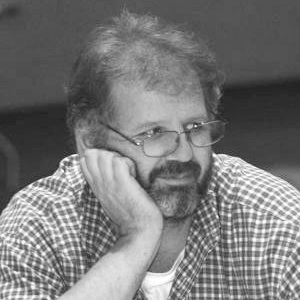
\includegraphics[width=1in,clip,keepaspectratio]{images/timm.jpg}}]{Tim Menzies} (Ph.D., UNSW)
is a Professor in CS at Morth Carolina State University (USA) and  the author of
over 200 referred publications. In terms of citations, he is one of the top 100 most
most cited
authors in  software engineering (out of 54,000+ researchers, see
http://goo.gl/vggy1). He has been a lead researcher on
projects for NSF, NIJ, DoD, NASA, as well as joint research work with
private companies. He teaches data mining and artificial intelligence
and programming languages. Prof. Menzies is the co-founder of the
PROMISE conference series (along with Jelber Sayyad) devoted to reproducible experiments in
software engineering: see http://openscience.us/repo. He is an
associate editor of IEEE Transactions on Software Engineering. the Empirical Software Engineering Journal, and the
Automated Software Engineering Journal.  For more information, see his web site http://menzies.us
or his vita at http://goo.gl/8eNhY or his list of publications at
http://goo.gl/8KPKA .
\end{IEEEbiography}


\begin{IEEEbiography}[{
\includegraphics[width=1in,clip,keepaspectratio]{images/davies1_gs.jpg}}]{Misty Davies}
(Ph.D. Stanford),is a Computer Research Engineer at
  NASA Ames Research Center, working within the
  Robust Software Engineering Technical Area.  Her
  work focuses on predicting the behavior of
  complex, engineered systems early in design as a
  way to improve their safety, reliability,
  performance, and cost. Her approach combines
  nascent ideas within systems theory and within the
  mathematics of multi-scale physics modeling.
For more information, see her web site http://ti.arc.nasa.gov/profile/mdavies
or her  list of publications at
http://ti.arc.nasa.gov/profile/mdavies/papers.
\end{IEEEbiography}



\clearpage
 \setcounter{page}{1}
\pagenumbering{Roman}
\section*{Reply to Reviewers}
\subsection*{Comments from the Associate Editor}

 I am recommending a major revision.  However please note that if you choose to submit a major revision, these changes must be made to the satisfaction of the reviewers in your next submission as we don't normally have two consecutive major revision decisions -- and I certainly can't recommend this a third time.
\begin{changed}
Thank you for the opportunity to resubmit. 
This draft makes the changes you indicated in the last review.
Please note that in this draft, all the changed material is shown in BLUE.

The current draft is not short and, if you want,
there is a way to reduce the size-- drop the three
tables ``maths models'' shown in the appendix. These
are well-documented in other publications.  Please
advise: drop or keep?
\end{changed}

The reviewers have recognized the efforts you've made but still raise some important concerns.  In particular could you please address the following.


1) Why did you not perform a comparison against your own previous work in ASE13/ICSE13 (IBEA) which you have shown to outperform the NSGA-II and SPEA2 baselines in this paper?   It doesn't make sense to use a lower baseline than the state of the art (especially when that is YOUR state of the art).

\begin{changed}


For more notes on our choice of comparison algorithms:
\bi
\item
See \tion{compares}: in summary, while there are many multi-objective algorithms out
there, many of these are ``frameworks'' not specific implementations.
So on the grounds of repeatability, it is better to compare against
NSGA-II and SPEA2 and not some generic framework like MOEA/D or PSO.
\item As to ``why don't we use the software product line examples from
our ASE13/ICSE13 papers?'', please see our comments in the next column.
\ei


\end{changed}

You need to build a convincing case that this can be
used to solve non-trivial Software Engineering
problems.  
\begin{changed}
To make that point, for this draft,
we added another SE study- based on Boehm's
software process modeling (see the one and a half page description
of XOMO in \tion{xomoIs}).


As for the ``non-trivial'' nature of our existing models,
please look at the following sections (the new text written in blue):
\bi
\item
The complexity of software requirements engineering in the context
of the large simulators in CDA is now defined more in \tion{cda}.
Note that our NASA colleagues requested us to work on CDA
since all their conventional methods were too slow and cumbersome (which is
evidence for the notion that GALE addresses an issue that is of
vital concern to some users of software).
\item
The ever-present ``magic weights'' problem is discussed in \tion{w};
\item
The problem of reasoning over agile systems is stressed in \tion{pom3pom3};
\ei

Not only that, but one of the authors (Krall)
spent months working on-site at NASA Ames Research Center to assemble the CDA model (in source,
the CDA model was not commissioned to be directly optimized nor was it clear which parameters could
or should be optimized).  This emphasizes another important part of SBSE: models must first be commissioned
so that inputs can be mapped to outputs (via evaluation).  For trivial models, this task would be simple, but
clearly, several months spent in commissioning is not a trivial matter.
\end{changed}

Similar to point \#1, why didn't you (for
example) include the case studies from previous work
in this evaluation?  
\begin{changed}
For notes on our choice of problem models:
\bi
\item
In \tion{abutsbse} we distinguish between a  ``classic SBSE'' problem
and certain specialized sub-types of problems. 
We then focus this paper on the classic problem (which we say means
``no knowledge of internal structure'').
\item
Further, 
in
\tion{compares}, we make the point that:
the ASE/ICSE13
papers on hierarchical software product line (SPL)
models is a different and specialized problem to the flat vector
decision space explored by the classic SBSE  problem solvers.
More specifically, 
the ``push,pull'' heuristics of the
ASE/ICSE13 papers would be of little benefit for ``classic'' problems
since, for this paper, we assume
no knowledge of internal dependencies.
\ei
FYI- there are now graduate students at NC state
working on meta-meta-heuristics for matching problem
types to algorithms. This is a \underline{HUGE}
task-- and one that will take sometime
before we can offer anything definitive for a TSE
article.  
\end{changed}
At the very least you need to
apply your technique in a way that convinces that it
is relevant for solving real SE problems.
\begin{changed}
Just as an aside- did you see Andreas Zeller's recent Facebook
discussion on ``what is a real SE problem?''. He was complaining that
if everything new is considered ``not SE'' then SE will become the
place of dull problems that are already solved.

(By the way, we expand a little more on these ``new SE problems'' in Question 1
of our new ``Frequently Asked Questions'' section in \tion{faq}.)

As to our applicability to ``real problems'',
we added yet another real world model to this paper (the XOMO work).
Also, as stated above, we explore these kinds of models
with these kinds of tools because
real people using real model-based software for real-world
applications are always pleading with us to make the whole
process really much simpler. Really.


\end{changed}


Please justify the quality metrics you use for evaluation purposes.

\begin{changed}
It is fair complaint to say that the prior draft did not apply
typical multi-objective evaluation procedures.   Accordingly, this draft corrects that problem: along with Equation~1
and number of evaluations, we also use the ``spread'' and ``hypervolume'' measures that are more standard
in the field.





\end{changed}

\subsection{Reviewer 1 Comments}

The paper is very well written with the proposed algorithm explained in detail and the results analyzed thoroughly.

The empirical study was conducted in a comprehensive fashion; it is also a plus to have made the implementation and the datasets publicly accessible.
\begin{changed}

Thank you for those kind remarks.
\end{changed}
Despite the above positive points, the paper has a
couple of shortcomings. The most noticeable one is
that good, and surprisingly good, results are
achieved based on only one heuristic, namely,
splitting the solution space into equal-sized
subsets and evaluating the farthest points in each
subset. On one hand, the results seem empirically
valid. On the other hand, the * why * is weak. The
best rationale that the author provide is that GALE
understands and exploits the shape of the Pareto
frontier. However, how do we know the shape of the
Pareto frontier is linear? Even if so, how do we
know the shape can be reasonably represented by
"east-west"? Both theoretical and empirical
arguments are needed to offer more substantial
insights into * why * GALE's simple heuristic works.

\begin{changed}
This is a fair comment that addresses an issue
overlooked in the previous draft. In this draft, in
\tion{faq} under the heading {\em Question 3}, we
note that GALE exploits an assumption that is
implicitly endorsed by the rest of the community,
but not exploited directly.
\end{changed}


The paper also contains several grammar-related issues: listed below.

\begin{changed}
Fixed (thanks for the pointers).
\end{changed}

\subsection{Reviewer 2 Comments}




The core contribution of this work is a novel MOEA;
its application to two software engineering problems
is merely incidental. As such, this work should
really be submitted to a journal on evolutionary
computation such as IEEE Transactions on
Evolutionary Computation where it would get more
expert reviews
\begin{changed}
We think it unfair to say that SE lacks  experts in evolutionary
methods. For example, the associate editor managing
this paper is one of them (and, we suspect,
so is Reviewer 4).

Also, we would say that this paper results from good software
engineering research since
the success
of GALE is due more to good software engineering than
anything else.
As software engineers,
the authors find an under explored area of the optimization
software literature and built the experiments to explore
that region.  
So we would say that GALE is an example of K.I.S.S. and YAGNI.
Further,  this work is less of an {\em algorithms} paper
than an {\em engineering} paper. 


\end{changed}


I am not an expert in MOEA but I
understand there has been much work in improving
MOEA since NSGA2 and SPEA2 both published more than
10 years ago. None of the more recent work in that
area is referenced in the paper,

\begin{changed}
We agree-- That is a  fair criticism of the last draft. 

This draft has more comments on other algorithms in 
\tion{algo} and
\tion{decomp}.
\end{changed}

GALE should
really be evaluated against or at least related to
the state-of-the-art in MOEA instead of just against
the two mostly widely-used algorithms in SBSE.

\begin{changed}
FYI- we tried to find some generally recognized state-of-the-art
(by emailing leading figures in the field) but we found no consensus.

And your general point is well made: we needed a better
discussion on why we used our comparison algorithms.
That has been fixed in this draft- see  \tion{compares}.
\end{changed}

 MOEA are of course of interest to software engineers
and thus have a place in TSE ...

\begin{changed}
On this point, we completely agree.
\end{changed}

... but for a TSE paper I
would expect the main contribution to be specific to
software engineering, for example by showing that
GALE can solve real SE problems faster and better
than previous approaches or that it can solve SE
problems that could not be solved before.
\begin{changed}

This is a
well known issue in SBSE that has resulted in
numerous attempts to define a set of canonical
problems that researchers can use to benchmark their
methods. We used some of those models in the previous draft
and reviewer 4 pointed us to some more, and these are
included in this draft.

Now we suspect Reviewer 2 would find those
canonical problems are too small to express
standard business knowledge. Hence this paper explores much
larger SE models.

FYI: we spent much time considering the choice of a larger
model that we explored.
Some researchers explore the
next-release planning problem but, at the advice of
Mark Harman, we stayed away from that one since (as
he warns) it is very hard to get accurate data on
those kinds of problems. 
In other work, in
ICSE/ASE13, we explore software product lines but these are highly untypical
of the standard SBSE problem.
For our notes on those models, and why we did not
use them here, see  \tion{abutsbse} 
and
\tion{compares}.

\end{changed}

 This is not achieved by the paper in its current
 form. The two SE problems to which GALE is applied
 are new to this paper and due to their short
 presentations are hard to understand and validate
 as real, significant SE problems (they possibly are
 real and significant but need more explanation). 

\begin{changed}
To address these issues, this paper takes more care
to situate the studies in an SE content (see the BLUE
notes in the following sections):
\bi
\item
Since the last draft, we added one
more SE model to this study-- see the one and a half
pages devoted to the XOMO software process models in \tion{xomoIs}.
\item
The problem of reasoning over agile systems is stressed in \tion{pom3pom3};
\item
The complexity of software requirements engineering in the context
of the large simulators in CDA is now defined more in \tion{cda}.
Note that our NASA colleagues requested us to work on CDA
since all their conventional methods were too slow and cumbersome (which is
evidence for the notion that GALE addresses an issue that is of
vital concern to some users of software).
\ei
\end{changed}

I
 would be more easily persuaded by this work if GALE
 was evaluated using previously published SBSE
 optimisation problems (for example some of the
 previous work of the second author, some
 requirements optimisation problems, or some testing
 problems). 
\begin{changed}
At your suggestion,
for this draft, we have added in a case study optimizing decision making in software processes in  \tion{xomoIs}.

\end{changed}

Other more specific comments:

I do not understand and I am not convinced by the measure of quality in Section 5.2. One technical presentation issue is that in Section 5.2, the loss function takes as arguments two *sets* of solutions (the final population and the initial population) whereas in Equation 1, the loss function takes as arguments two *individual* solutions x and y. So there appears to be a type-checking error here. 

\begin{changed}
Our mistake. We actually compare the means of the populations.
And we added more text to explain that point in \tion{eval}.

\end{changed}

Some examples illustrating Equation 1 would also have been very useful to help my understanding of this loss function. More importantly, if we abstract away from the technical details, I would have liked to see some justification for using this function as a measure quality. 
\begin{changed}
For a detailed justification of that loss measure, there is this text in \tion{cdom}:

\begin{quote}
 Recently, Sayyad~\cite{sayyad13a} studied binary domination for MOEA
with 2,3,4 or 5 objectives.  Binary domination performed as well as anything else
for 2-objective problems but very few good solutions were found for
the 3,4,5-goal problems.  The reason was simple: binary domination  only returns
{\em \{true,false\}}, no matter the difference between $x_1,x_2$. As the objective
space gets more divided at higher dimensionality, a more nuanced approach is required.
\end{quote}

\end{changed}

Comparing the solutions generated by an algorithm against those of the initial population amounts to comparing it against a random search. Is this a good way to measure quality? I believe an alternative approach used by the MOEA community is to compare the generated solutions against some reference Pareto-front where the reference Pareto front is obtained from all executions of all algorithms. 
\begin{changed}
Such frontiers are not available for all the complex models we explore here.
\end{changed}

Additionally, MOEA are usually evaluated not only
by their relation to the reference pareto-front but
also by the spread of their solutions. The
discussion you give in the paper why standard
measures of spread are inappropriate for GALE is not
satisfying (or I did not understand it well enough).
In summary, I believe the evaluation of quality
needs better justification and possibly to be redone
entirely.

\begin{changed}
Thanks for this remark. Now we use spread in the results section.
\end{changed}



Section 2.5 is hard to understand. It lacks
definition and examples for most of its key
concept. In the first paragraph, it is not clear
what you refer to when you talk about "decisions",
"dimensions" and "data". Figure 4a is useless
because it does not illustrate how WHERE decides
which car goes into what cluster. Using a simple SE
example (e.g. a basic requirements optimisation or
test optimisation problem) instead of a car
selection problem would help make the description
more relevant and comprehensible to software
engineers.


\begin{changed}
At your suggestion, we have {\em considerably} simplified that section (and discarded that
overly complex example).
\end{changed}

The sections introducing the POM3 and CDA models are
distractions from the core contribution of the
paper. These sections are too long if their purpose
is to introduce models against which to evaluate
GALE and too short to actually understand the models
and validate them as real significant SE
problems. Each model probably requires a separate
full-length paper to introduce its context, present
the decisions it is intended to support, and justify
its equations, assumptions and choices of
objectives.

\begin{changed}
That was our mistake. This draft does a better job of 
recording the papers that document those models. 

To be precise, each section CDA, XOMO, POM3 starts with a list
of background papers:

\bi
\item POM3: \cite{port08,me09j,1204376,turner03};
\item XOMO: \cite{me07f,me09a,me09e};
\item CDA:  \cite{Kim2011,Pritchett2011,Feigh2012,Kim2013,Pritchett2013}.
\ei
\end{changed}


\subsection{Reviewer 3 Comments}

Recommendation: Author Should Prepare A Major Revision For A Second Review

Comments:
Overall I find the paper well written and focused. It seems to have gone through a major revision and improvement over the previous draft.
\begin{changed}
Thank you-- we spent much time on that draft, and on this one as well.
\end{changed}

My comments and concerns are more from a methodological point of view. This is the reason why marked it as a major revision. Should my concerns be properly addressed the paper would be fit for the inclusion in TSE.

First, the paper compares GALE against two other commonly used MOEA's: NSGA-II and SPEA2. However, previous recent work by one of the co-authors, presented in ASE13 and ICSE13, strongly suggests that IBEA algorithm outperforms NSGA-II and SPEA2. This begs the question: Why not include IBEA in your comparison if your own previous work has shown it performs better than the other two selected algorithms?

\begin{changed}
The associate editor asked the same question. Please see our replies
to her question, above.
\end{changed}

Second, along the same lines. In those previous
publications, there are several case studies from
the realm of Software Product Lines. The question
is: Why not use also those case studies to further
evaluate your new algorithm?


\begin{changed}
Please see our comments on this issue, above, in our discussion with the
associate editor.
\end{changed}
In my opinion, addressing these two previous point can strenghten your results and provide a more rounded context to your GALE work.

Considering the little time it takes to run GALE and the other algorithms in your models, using 20 runs seems to be too little. Usually at least 30 runs are ok, but as Arcuri and Briand suggest in [1] even more runs ought to be expected.

\begin{changed}

We certainly agree that most of the methods used for
search cite their reason for performing repeats of
the experiments: the results are based off of
stochastic processes and it is important to rerun
the tool for statistical validity~\cite{1334912}.
However it is disputed as to how many repeats should
be performed, ranging from as few as 5 and sometimes
as high as 100 and even 1000~\cite{krall14f}.

(The numbers in this sentence
come from a lit review we started, prompted by this reviewer comment. We thank
this reviewer for this comment since that lit review is maturing nicely and should be ready for submission, soon.
For some preliminary notes, see~\cite{krall14f}.)

Note that a statistical case can be made for {\em not} performing too many repeats~\cite{isre.2013.0480}
(the dreaded p-Value problems).
Pragmatically, a small sample size is desired unless
the search can be repeated dozens of times per
second.  While a sample size of 1 to 5 is
fundamentally too small to identify any pattern or
statistically significant differences in the data, a
sample size of 10 may still be questionable, but
from personal findings, a sample size of 20 seems to
be no different than a sample size of 50.  Hence, a
sample size of 20 is a good medium between too-small
and too-large.


\end{changed}

Also based on [1], there is no report of effect size measures such as A12 which are fundamental when comparing search based techniques.

\begin{changed}
Thank you for that comment: this draft makes extensive use of A12.
\end{changed}

Regarding your evaluation. You measure the improvement from an initial randomly-generated population to the final frontier as you called it. My question here is: Do the evaluation of all algorithms start from the same initial population(s)? I cannot tell from the text. If not, then, is it a fair comparison if they start from a different population?

\begin{changed}
Thank you for that comment: you are correct- all our experiments start from the same initial population
(we added a comment on that at the end of \tion{expexp}).
\end{changed}

I do not agree with the point that "it can be better
to study GALE's spread visually rather than
...". Visualizations can be complementary to the
proper math analysis but not a substitute. I
strongly suggest that the evaluation/analysis is
made both ways, mathematically and visually, if you
claim that a visualization can help to illustrate
your point.
Regarding the other quality indications (HV and GD). Sure there is no perfect measure, all of them have both pros and cons. However, I fail to see any strong reason why you chose not use them as complementary measures to assess your algorithm.

\begin{changed}
We quite take your point. This draft now uses hypervolume and spread.
\end{changed}

Minor comments:

* The values depicted in Figure 4 are not clear what they mean. Are they values from an independent variable?


\begin{changed}
That figure has been dropped since several reviewers had issues with it.
\end{changed}

* Perhaps I am misunderstanding something. But in Figure 18 for the ZDT1 model, you have highlighted both GALE and SPEA2 with values 80\% and 82\% respectively. But shouldn't these values be equal or just one of them being highlighted?

\begin{changed}
On that row, in the last draft,
only the 87\% is significantly different to the other numbers.

And, when we re-ran the experiments and the stats for this draft, that effect
went away (but the main effect remained; i.e. GALE usually found most improvement).
\end{changed}

\subsection{Reviewer 4 Comments}

Recommendation: Author Should Prepare A Major Revision For A Second Review

Comments:
This is a good paper in general, but there are a few loose ends that need to be tightened. Some are more major than others. I hope they are of some use to the authors in revising their work.


\begin{changed}
Thank you for those comments.
\end{changed}

"When MOEAs explore too many options, they are slow to use and hard to
comprehend." This is very vague and is true for almost any search
algorithms, not specific to MOEAs. Please revise.



\begin{changed}
You are correct. We changed that, as per your comment, to ``automatic tools''.
\end{changed}


"Given cloud computing,..." I don't think you have to use cloud
computing to exploit the benefits from SBSE. The advancement in more
efficient algorithms can be more important than the availability of raw
computing speed.


\begin{changed}
You are correct. We changed that, as per your comment, to ``Given recent advances in computing hardware..''
\end{changed}

I don't think Figure 1 and the following sentence, "For example, Figure
1 shows an SBSE tool that has rejected thousands of less-than-optimal
solutions (shown in red) to find a smaller number of better solutions
(shown in green).", add much to the paper. They should be removed.


\begin{changed}
You are correct. We deleted that figure and its associated text-- and the paper's introduction is now much better for it.
\end{changed}

 The 3rd paragraph in Introduction (page 1): The paragraph
does not look very rigorous. The
point it wants to make can be made in a sentence or two. I would suggest
deleting the paragraph and replace it by a couple of sentences only.


\begin{changed}
You are correct. Once again, ``less is more''.
We deleted that para-- and introduction is better for it.
\end{changed}

I'm not sure of the sentence "One standard method to reduce the
space of solutions is to find the Pareto frontier ..." Pareto fronts are
usually used to explore trade-off among conflicting objectives, not
reducing the search space.


\begin{changed}
Good point. We changed that to 
``One way to simplify the task of understanding these
algorithms is to focus on the {\em Pareto frontier}.''
\end{changed}

This sentence needs revision: "GALE is an evolutionary learner where
solutions in the next generation are mutations of the previous
generation." because the next generated is always mutated from the
previous generation for all evolutionary algorithms, let alone MOEAs. The
sentence does not really explain the novelty of GALE precisely and
clearly.

\begin{changed}
Good point. We removed that text. Now the intro has a very clear and short
dot list describing GALE.
\end{changed}


The two research questions towards the end of Section 1 need some
refining, proably with one or two supplementary questions. As we known,
there is no free lunch in search. One should not expect a clear yes/no
answer to these two questions. In this case, it's essential to understand
{\em when} the answer would be yes/no. In other words, it's essential to
understand for which type(s) of SE problems GALE is faster/better. Without
bringing the SE problems into the research questions, we run the risk of
drawing biased conclusions that may not always be true.


\begin{changed}
Good point. We handled that with some clarification answers to a ``Frequently
Asked Questions'' section on page2. Please check our ``Question2'': does it
address the issue you raise above?
\end{changed}

In Section 2.1, the authors gave Figure 2 to summarize the related work,
I don't find this useful or satisfactory, because it missed a lot of
important work, both more recent and old papers, on MOEAs for SE.


\begin{changed}
Good point. We removed that table and instead referenced the reader 
to recent survey articles~\cite{harman12abc,harman14}.
\end{changed}

Overall, I'm unsure Section 2.1 is really needed for this paper. It
talked very generically about SBSE, while the focus of this paper is on
MOEAs and their applications to SE. I think the paper would be sharper
without the distraction of Section 2.1.


\begin{changed}
Good point. We removed that section, started with MOEAs (but we
did a subsequent section \tion{abutsbse} about SBSE since other reviewers
wanted to understand why we explored these problems ant not others.
\end{changed}

In comparison to Section 2.1, Section 2.2 on MOEAs is too thin. There
should be a better overview of different MOEAs for SE, since this is the
topic of this paper.


\begin{changed}
Good point. Please check \tion{abutsbse}
and \tion{algo} and \tion{decomp}.

Now, we suspect that you will have issues of the brevity of those sections
but please be aware of how {\em long} this paper is. After much writing
and rewriting, we elected to put fewer introductory details into the start
so we can do more experiments at the end. 
\end{changed}

Given the discussion in the first paragraph of Section 2.3, the authors
might want to consult the literature about $\epsilon$-dominance.


\begin{changed}
EXCELLENT POINT!!!  Spot on. Important related work. Please see  \tion{decomp}.

\end{changed}

Two major performance measures used by MOEA researchers are convergence
(to the Pareto front) and diversity among non-dominated solutions. It
appears that Section 2.3 rarely mentions the diversity issue explicitly
when discussing MOEAs. Only convergence was emphasised. Any particular
reasons? I thought diversity is very important to software managers in
understanding different trade-off.


\begin{changed}
EXCELLENT POINT!!!  We have explored spread extensively in this draft.
And what we discovered was that GALE does {\em very well} on spread.

So thanks for that comment.
\end{changed}


In section 2.4: "These models allow for an extrapolation between known
members of the population." I guess the authors might mean
"interpolation"?
\begin{changed}
Good point. We changed that to  ``These models allow
for an extrapolation from \ADD{known members of the
population to new and novel members}.''
\end{changed}

I like the idea described in Section 2.4 (and [4]) very much.
It would be nice to point out explicitly the assumptions implied by such
approximation.


\begin{changed}
Good point. For a discussion on those assumptions,
see the end of {\textsection}2.7.

Actually, this was another spot-on comment. It turns out that those
assumptions are critical to the success of GALE.
\end{changed}

Unsure why Section 2.5 included so much details while Sections 2.3 and
2.4 did not. Was it because the novelty claims by this paper were built on
spectral learning?

\begin{changed}
Good point. We have reduced the complexity of that section.
\end{changed}


After reading through GALE in detail, as described by Section 3, I'm
very keen on knowing the diversity of the solutions found by GALE in
comparison to other MOEAs.


\begin{changed}
At your most excellent suggestion, this draft explores spread extensively.
\end{changed}

In Section 4.2.1, the benchmark functions used are considered to be
obsolete by the MOEA community because they are unable to reveal fully
different features of different MOEAs. The better and more recent ones are
the DTLZ and WFG benchmark sets.


\begin{changed}
Good point. We dumped many of the older models (e.g. Schaffer, which is clearly
obsolete) and made extensive studies on DTLZ. 

And the DTLZ results were very positive- see figure 15 and 16. GALE does much
better as the number of objectives and decisions goes up. Very nice result.
\end{changed}

The discussion on Page 11 of comparing NSGA-II and GALE can be misleading
because it looked at one or two objectives only in comparing NSGA-II and
GALE without comparing other objectives for this many objective
optimization problem. When comparing two MOEAs, we should use the dominance
relatoinship over all objectives, rather than looking at only a subset of
the objectives.
\begin{changed}
Good point and we concur. This draft dumps that discussion. And
we do a better job of studying our effectiveness across multiple objectives.
\end{changed}

In Section 5.3, I'm unsure of the answer to RQ2. The quality here seems
to mean Equation (1). There are two issues here: (a) If the metric of
Equation (1) is all that's important and compared against, one could
actually use a single objective algorithm to optimise Eq.(1) directly. (b)
For MOEAs, the comparisons should be based on the dominance relatoinship
over all objectives, rather than looking at only a subset of the
objectives. Otherwise the conclusions drawn are likely to be misleading or
flawed.
\begin{changed}
Good point and we concur. As shown in {\textsection}6, we evaluate on many objectives
now using composite measures such as spread and hypervolume.
\end{changed}


The MOEA community has already
developed better benchmark functions, e.g., DTLZ and WFG sets, in order to
evaluate how different MOEAs behave on different problems. Why not use
these benchmark problems to evaluate GALE, just like other MOEA developers
would do for their newly invented MOEAs?

\begin{changed}
We concur. We now use DTLZ extensively.
\end{changed}


The discussion in Section 6.4 confirmed my guess that GALE emphasizes
convergence to the pareto front only, but does not consider even
distribution of solutions, i.e., spread (or diversity). This indicates
that GALE has a different design goal from other MOEAs, which must
consider both convergence and diversity. As a result, it's unclear to me
that this paper is carrying out a fair comparison.


\begin{changed}
We concur. Now we make more use of spread and hypervolume.
\end{changed}

I'm a little confused by Figure 20. There are six red stars by GALE, four
of which are dominated by blus triangles (from NSGA-II). The paper said that
"... but in the y direction, it is GALE that extends further ..." However, the
extension seems to go towards the worse direction. I seem to have missed
something here. Some clarifications would be nice.


\begin{changed}
We concur. Now we make more use of spread and hypervolume.
\end{changed}


Figure 21 gave a good summary of the weakness of GD and HV. However, in
comparison with Eq . (1) used in this paper, HV would be a far more
appropriate measure for comparing MOEAs, if one is allowed to use only one
measure, as pointed out by existing MOEA literature. There are near linear
time algorithms for approximating HV effectively and efficiently.


\begin{changed}
We concur. Figure dumped.
\end{changed}

The conclusions drawn in Section 7 seem to be too strong and general, not
supported by the experimental studies in the paper. (a) The paper
emphasized GALE's approximation to the Pareto front. Unfortunately, this
was poorly done because GALE found only a few points, which could hardly
represent an approximate front. I appreciate that this is by design and
controlled by the "enough" parameter. The paper needs to have evidences to
show that GALE's solutions are approximating a front, not a few points
only. 


\begin{changed}
We concur- the previous draft was not good on this point.

What we say now (in the intro and conclusion is that)...
\begin{quote}
GALE’s truncated search explores a somewhat
smaller hypervolume of solutions than other optimizers.
Yet within that smaller volume, GALE’s careful directed
search is more spread out than other methods. More
importantly, on inspection of the raw objective scores,
we often find better results with GALE than with other
optimizers.
\end{quote}
Note that this conclusion would have been IMPOSSIBLE without you
pinging us to study spread. So thank you for that.
\end{changed}

It is very hard to understand (due to my limited knowledge) why an
MOEA should ignore diversity (i.e., spread in this paper) and focus on
convergence only, because this will lead to a non-dominated set that's
very unevenly distributed over different trade-offs. It seems to be
contraditory to the fundamental motivaions behind MOEAs. (b) When GALE
used two extreme points (poles) to approximate a part of the Pareto front,
isn't there an assumption that the real underlying Pareto front is smooth
between the two poles? It would be interesting to use benchmark functions
with non-smooth Pareto fronts to evaluate GALE. Some of the DTLZ and WFG
functions would be very useful for this, especially the authors claimed
"that GALEs superior performance is due to its better understanding of the
shape of Pareto frontier." This is currently not supported by factual
evidences in the paper.
\begin{changed}
Once again: spot on. The previous draft could not support that conclusion.

However,
we think that the new results on spread in this draft address this issue.

But what is your view?
\end{changed}

Just as a final thought, I wonder whether a bit more emphasis on the SE side, instead of on GALE, might help to enhance the novelty and significance of the paper. However, I leave it to the authors to decide and revise the paper.

\begin{changed}
Thanks for that comment. We added another ``SE'' kind of model (the XOMO stuff in \tion{xomoIs}).

Also, again at your suggestion, in this draft
we pushed back some of the experimental detail to the back while
pushing all the model descriptions earlier into the paper.
\end{changed}

\end{document}
